\documentclass[10pt,journal]{IEEEtran}

\usepackage{graphicx}
\usepackage{subfigure}
\usepackage{cite}
\usepackage[justification=centering]{caption}
\usepackage{makecell}
\usepackage{amsmath,amsfonts, amsthm}
\usepackage[ruled, linesnumbered]{algorithm2e}
\newtheorem{definition}{Definition}
\newtheorem{theorem}{Theorem}
\newtheorem{lemma}{Lemma}
\usepackage{booktabs}
\usepackage{xcolor}

\hyphenation{op-tical net-works semi-conduc-tor}
\hyphenpenalty=6000
 \tolerance=10000


\graphicspath{{./figures/}{./photos/}}

\begin{document}

\title{FishboneChain: A Scalable and Liquidity-Guaranteed Crowdsourcing Platform based on Multiple Child Chains}

\author{Wentuo Sun, Kaiping Xue,~\IEEEmembership{Senior Member,~IEEE,} Meiqi Li, Xinyi Luo,~\IEEEmembership{Graduate Student Member,~IEEE}
    \thanks{W. Sun, K. Xue, M. Li, and X. Luo are with the School of Cyber Science and Technology, University of Science and Technology of China, Hefei, Anhui 230027, China.}

	\thanks{Corresponding Author: K. Xue (kpxue@ustc.edu.cn).}
}


\IEEEtitleabstractindextext{%
    \begin{abstract}
    The integration of blockchain with crowdsourcing improves data security, reduces single-point failure risks, and enhances trust and traceability in the system. However, this integration also leads to scalability issues because of the decentralized consensus mechanism of blockchain. While multiple chain architecture can enhance system throughput and offer functionality extensions, they often require complex token locking and release mechanisms to prevent double-spending attacks. This leads to a significant portion of funds being locked, thereby reducing overall fund liquidity.
    In this paper, we propose FishboneChain, consisting of one main chain and multiple child chains. Specifically, we address the scalability issue by leveraging child chains to offload the crowdsourcing task result submission and verification transaction pressure from the main chain, while each child chain can deploy various crowdsourcing protocols to enhance the functionality. Furthermore, we design a fund management contract and periodic task settlement mechanism, which allows requesters to lock a single fund on the main chain to manage task status across multiple child chains, thereby reducing the locked fund percentage and improving fund liquidity. Our scheme satisfies the security requirements of a crowdsourcing platform, such as fund security, robustness, and double-spending resistance. Performance analysis shows our scheme can improve the system throughput to 100 times that of the main chain and maintain the locked fund percentage below 20\%.
    \end{abstract}

    \begin{IEEEkeywords}
        Blockchain, child chain, smart contract, crowdsourcing, scalability
    \end{IEEEkeywords}

}

\maketitle
\IEEEdisplaynontitleabstractindextext
\IEEEpeerreviewmaketitle

\section{Introduction}
Crowdsourcing serves as a widespread methodology for task completion and data collection, leveraging the collective intellect and resources of large communities. The realm of business features numerous examples of crowdsourcing applications today. A notable example is Wikipedia \cite{wikipedia}, a well-known crowdsourcing platform that enables users to engage with the system by responding to queries posed by fellow users. Other crowdsourcing platforms with extensive user bases and large-scale datasets include Mechanical Turk (MTurk) \cite{MechanicalTurk} and Waze \cite{Waze}. In conventional crowdsourcing systems \cite{wu2014smartphones, to2016differentially, wang2019optimization, xiao2016online, miao2017lightweight}, a centralized and trusted third-party structure characterizes the crowdsourcing platform. Users usually need to submit comprehensive personal information and task-related data to the platform. Requesters post their tasks along with their rewards on the platform. Workers then complete these tasks according to the requirements and submit the generated data to the platform. The platform conducts validation checks on the task data and dispenses appropriate rewards to the workers. However, centralized crowdsourcing platforms face trust and security issues. Users must trust that the platform fairly allocates tasks to workers, settles payments equitably, and refrains from misappropriating users' remaining funds. Additionally, centralized platforms are vulnerable to single points of failure, such as Distributed Denial-of-Service (DDoS) such as link-flooding attacks \cite{huang2024you}, which can render them unable to provide services.

To address the trust and security issues of centralized architectures, researchers introduced blockchain technology featuring decentralized and publicly verifiable smart contracts \cite{an2022ppqc, li2018crowdbc, lu2018zebralancer}. In this shift, the conventional centralized server is replaced by a blockchain equipped with self-executing smart contracts. In a blockchain-based crowdsourcing system, platform maintenance, including data verification and storage, task assignment and fund transactions, is shared among all miners. Consensus algorithms like Proof of Work (PoW) \cite{nakamoto2008bitcoin} and Proof of Stake (PoS) \cite{king2012ppcoin} enhance resilience, allowing the system to function even when a small fraction of miners are malicious. However, despite the clear benefits of blockchain integration, persistent issues still affect the viability of blockchain-based crowdsourcing systems, particularly regarding scalability and compatibility.

In terms of scalability, the decentralized consensus mechanism of blockchains, such as PBFT \cite{castro2002practical} and RAFT \cite{ongaro2014search}, poses challenges for achieving high throughput. This is especially apparent in data-intensive scenarios like crowdsourcing. In crowdsourcing scenarios, large amounts of data need to be processed and validated quickly. However, the consensus mechanism of blockchain is a performance bottleneck, preventing the system from meeting real-time and high concurrency requirements. Furthermore, compatibility issues pose another major challenge for blockchain-based crowdsourcing platforms. These platforms must continually expand their functionalities to keep pace with the evolution of crowdsourcing scenarios. In the meantime, a number of well-established crowdsourcing protocols designed for diverse scenarios exist, including mechanisms for task assignment \cite{zheng2015qasca, wang2017multi, bhatti2020approximation} and incentive structures \cite{zhang2014free, yang2015incentive, wang2020socialrecruiter}, among others. Last but not least, the open nature of blockchains reveals all smart contracts and data, necessitating the design to preserve users' privacy, as shown by works such as \cite{qiu2020location, yuan2019priradar,wang2019towards, zhang2021enabling, cai2019towards}.

In recent years, numerous technologies are proposed to address the performance scalability issues of blockchain, including sharding \cite{luu2016secure,li2024secure,li2025s3voting}, off-chain channels \cite{poon2016bitcoin,luo2024crosschannel}, and sidechain or child chains \cite{poon2017plasma}. In these protocols, sharding primarily improves the main chain's throughput by processing transactions in parallel, thus requiring all shards to follow a unified protocol. Off-chain channels enhance throughput and reduce transaction costs by offloading the transaction verification process from the main chain to an off-chain environment, which can be verified by both parties. They only submit the final results of multiple transactions to the main chain. As a result, off-chain channels are typically protocols between two parties that face challenges in supporting protocol expansion. Sidechains and child chains differ in key aspects. They also offload the complex and massive crowdsourcing task result submission and verification from the main chain to the sidechain or child chains, improving overall throughput. Furthermore, sidechains and child chains are blockchains that can deploy specific protocols based on particular crowdsourcing requirements, thereby enabling functional expansion. Compared to sidechains, child chains have less independence and lower security risks because child chains rely more on the main chain for security guarantees. Therefore, child chains are the most suitable solution in crowdsourcing scenarios, offering scalability and compatibility while ensuring security.

However, child chains also have their own security issues. Given the relatively lower number of miners on a child chain compared to the main chain, adversaries can more easily compromise a child chain, leaving it incapable of delivering dependable services. Furthermore, the failure of timely state synchronizations between the main chain and child chains can open avenues for double-spending attacks, compromising fund security. To resist double-spending attacks within multiple blockchain architectures, current schemes require users to lock funds on the main chain when engaging with a child chain to acquire tokens for transactions on the latter. However, in crowdsourcing scenarios, where users often post tasks across various child chains to collect multidimensional data, a significant amount of funds can become locked in these child chains. This will restrain fund liquidity within the crowdsourcing platform, burdening users with complex and costly fund management across multiple blockchains.

To address the scalability issue in blockchain-based crowdsourcing platforms and the fund liquidity issue in multiple chain architecture crowdsourcing platform, we propose FishboneChain: an innovative crowdsourcing platform that is designed for scalability, compatibility and fund liquidity, built on a main chain and multiple child chains. We introduce a strategic separation of fund flow and data flow within the crowdsourcing process. Specifically, the tasks of data submission, verification, and storage are delegated to child chains, while the critical fund settlement operations are conducted on the main chain. In this way, we enhance the platform's throughput capabilities and ensure fund security. We also institute a synchronization mechanism during the periodic pay bill phase of the crowdsourcing process. This synchronization links the security of child chains to the main chain, mitigating potential security vulnerabilities stemming from disparate states. Furthermore, we present a new fund management contract that allows users to post tasks across multiple child chains utilizing a single locked fund. This can protect users against double-spending attacks and enhance fund liquidity on the platform. Although our primary focus is on platform-level scalability, security and fund management challenges, the FishboneChain platform also provides sufficient flexibility to address more granular security issues within the crowdsourcing process, such as free riding and potential data abuse. The periodic task settlement mechanism allows requesters to periodically evaluate task execution results and terminate tasks if necessary, limiting potential losses. Additionally, the FishboneChain structure is compatible with various existing incentive mechanisms and data quality verification schemes, which can be implemented by child chain miners to prevent malicious behaviors by workers.

Our main contributions are summarized as follows:

\begin{itemize}
    \item We propose the FishboneChain architecture, including one main chain with multiple child chains. We design a strategy that separates the fund and data. All financial transactions are conducted on the main chain, while the child chains are responsible for executing crowdsourcing tasks and validating results. In the meantime, the child chains can deploy specific crowdsourcing protocols based on crowdsourcing requirements to enhance the compatibility of the platform.
    \item To ensure fund liquidity, we develop a periodically free-lock fund management scheme enacted as a fund management contract (FMC) on the main chain. This scheme allows requesters to automate both fund management and task activation, preventing double-spending attacks across multiple child chains.
    \item We conduct security analysis on child chains, funds and the platform.
    The experimental results demonstrate that we can increase the platform's throughput to 100 times that of the main chain. In terms of fund liquidity, we can maintain the locked fund percentage at 20\% at least.
\end{itemize}

The rest of this paper is organized as follows. In Section \ref{section:related_work}, we present the related works about blockchain-based crowdsourcing and child chains. The preliminaries of blockchain, smart contracts, and child chains are given in Section \ref{section:preliminaries}. In Section \ref{section:system_model}, we introduce the security assumption, design goals, and the main components of the system. The description of our proposed architecture is given in Section \ref{section:solution}. We analyze the security of the proposed architecture in Section \ref{section:security_analysis}. In Section \ref{section:performance_analysis}, we show the evaluation results of a series of experiments, and finally, we conclude and discuss the future work in Section \ref{section:conclusion}.

\section{Related Work} \label{section:related_work}

In this section, we review existing crowdsourcing platforms and blockchain-based solutions, examining their strengths and limitations in addressing security, privacy, and scalability challenges. This comprehensive analysis provides the foundation and motivation for our proposed FishboneChain architecture.

There are many actually deployed crowdsourcing platforms, such as Amazon MTurk~\cite{MechanicalTurk} and Waze~\cite{Waze}. Despite their success, these platforms, due to their centralized architecture, are prone to single-point-of-failure problems. In addition, users need to have complete trust that the platform does not have security issues such as data tampering and privacy leakage.

To address the security and trust issues inherent in centralized architectures, numerous blockchain-based crowdsourcing solutions are proposed. These solutions primarily focus on aspects such as privacy preservation\cite{lu2018zebralancer,zhang2021enabling}, incentive mechanisms\cite{tong2024privacy}, and task allocation\cite{wu2024vp} within the crowdsourcing process. Lu \textit{et al.} \cite{lu2018zebralancer} proposed ZebraLancer, a blockchain-based anonymous crowdsourcing system, to enhance privacy through the common-prefix-linkable anonymous authentication. Zhang \textit{et al.} \cite{zhang2021enabling} proposed a proxy-free privacy-preserving and federated crowdsourcing system via rewritable deterministic hashing and puncturable encryption technique. Tong \textit{et al.} \cite{tong2024privacy} proposed an incentive mechanism based on reverse auction and implemented as smart contracts in blockchain. Wu \textit{et al.} \cite{wu2024vp} proposed a public verifiable privacy-preserving task-matching scheme for blockchain-based crowdsourcing.

Multiple child chain architecture can solve the scalability and compatibility issues in crowdsourcing scenarios by flexibly adjusting the number of child chains and designing child chain parameters. Zhu \textit{et al.} \cite{zhu2019zkcrowd} proposed a hybrid blockchain-based crowdsourcing platform named zkCrowd, which uses a public chain and multiple private subchains, where all public tasks performed on the public chain and private tasks performed on newly established private child chains. Wan \textit{et al.} \cite{wan2022hibechain} proposed an architecture that consists of multiple permissioned blockchains that form a hierarchical tree structure. However, directly applying this architecture to crowdsourcing scenarios still faces several challenges. Multi-chain platforms typically require users to lock a certain amount of funds on the main chain before joining a child chain in exchange for corresponding child chain tokens. While this mechanism prevents double-spending attacks that exploit delays in cross-chain state synchronization, it also results in a large amount of capital being locked on the main chain, reducing overall liquidity and capital efficiency. Secondly, due to the relatively small scale of maintainers for child chains, there is an increased possibility of child chains being attacked, potentially leading to asset losses and affecting user trust and platform stability. Finally, we present a table comparing the FishboneChain solution with existing crowdsourcing solutions in Table ~\ref{tab_solutions_comparison}.

\begin{table}[!ht]\centering
    \caption{Comparison with existing crowdsourcing platforms.}
    \label{tab_solutions_comparison}
    \resizebox{0.94\linewidth}{!}{
    \begin{tabular}{lcccccccc}
    \hline\hline
                     & \makecell[c]{\cite{Waze} \\ \cite{MechanicalTurk}}   &  \makecell[c]{  \cite{lu2018zebralancer} \\ \cite{zhang2021enabling}}    & \makecell[c]{\cite{tong2024privacy} \\ \cite{wu2024vp}}  &\cite{zhu2019zkcrowd}   & \cite{wan2022hibechain}     & FishboneChain$^{\text{ours}}$ \\
    \hline
    Decentralization        &N      &Y     &Y       &Y        & Y         &  Y
    \\
    Privacy Preservation    &-      &Y     &Y       &Y        & Y         &  compatible
    \\
    \makecell[l]{Data Quality
    \\ Validation}          &-      &N     &Y       &N        & N         &  compatible                      \\
    Incentive mechanism     &-      &N     &Y       &N        & N         &  compatible                      \\
    Scalability             &-      &N     &N       &Y        & Y         &  Y                      \\
    \makecell[l]{Child Chain
    \\Security}             &-      &N     &N       &N        &N          & Y     \\
    \makecell[l]{Flexible Fund
    \\Management}           &-      &N     &N       &N        &N          & Y  \\
    \hline\hline
    \end{tabular}}
\end{table}

\section{Preliminaries}\label{section:preliminaries}
In this section, we introduce the concepts related to our FishboneChain architecture, including blockchain, smart contract, and child chain.

\subsection{Blockchain and Smart Contract}

The concept of blockchain was first introduced by Satoshi Nakamoto in 2008 \cite{nakamoto2008bitcoin} as a foundational component of the Bitcoin cryptocurrency. The blockchain serves as a public transaction ledger, recording a continuously expanding list of blocks, each containing a set of transactions. These blocks are interlinked using hashes of the preceding blocks. A blockchain is usually managed by a peer-to-peer network that collectively adheres to a predetermined consensus protocol. Public blockchains are permissionless and accessible to anyone on the Internet. Private blockchains are permissioned and possess an access control layer. The owner exercises control over network participation and the consensus process.


Smart contracts are executable programs that reside within a blockchain. They depict complex logic by translating common processes into code and serve as the implementation of contract-based agreements, functioning as self-executing digital contracts within a secure environment. Verified by network peers, these contracts operate autonomously without the need for intermediaries. The decentralized, immutable, and programmable nature of blockchains provides an ideal environment for deploying smart contracts. Currently, a variety of blockchain platforms support smart contracts, expanding their applications beyond cryptocurrency trading to many other fields, such as securities trading, financial data recording, crowdfunding, and more. Examples include Ethereum \cite{buterin2014next} and Hyperledger Fabric \cite{androulaki2018hyperledger}.


\subsection{Child Chain}

An illustration of a child chain architecture can be found in Ethereum Plasma \cite{poon2017plasma}, which is described as a ``Blockchain in Blockchain". This innovative framework introduces a recursive parent-child structure as an effective solution to scalability and functionality challenges. In the context of Ethereum Plasma, a child chain is generated under the Plasma chain. This child chain processes transactions autonomously and transforms all transactions in the generated block into a single Merkle root hash. Then, write it to the parent chain.

At the beginning of the process, it is similar to the off-chain method. Initially, the process resembles an off-chain approach, with the Plasma chain operating as the parent. The newly created child chain behaved like a conventional blockchain. This child chain's transactions are archived in the parent chain as Merkle root hashes. Verification of blocks is accomplished through a fraud-proof mechanism in smart contracts. This approach allows anyone to participate in the verification process. The child chains are very efficient because only the Merkle tree root of the child chain is stored on the parent chain. The parent chain can divide its functions into multiple child chains, which in turn enables the extension of its functionality. This fosters flexibility and scalability of the blockchain, allowing it to adapt to changing requirements and evolving use cases.

\section{System model, security assumptions and design goals}\label{section:system_model}

In this section, we describe the system model, the security assumptions, and the design goals of FishboneChain.

\subsection{System Model}

As illustrated in Fig.~\ref{fig:FishboneChain_architecture}, our system comprises three roles: miners, who maintain the main chain and the child chains; requesters, who publish tasks on different child chains; and workers, who execute these tasks. The combination of one main chain with multiple child chains forms a structure resembling a fishbone. Hence, we name our scheme ``FishboneChain''. To process crowdsourcing tasks, the main chain records all relevant task information and oversees fund transactions using fund management contracts (FMCs). Each child chain only handles data-centric tasks in the crowdsourcing scenario, including data submission, verification, and recording. Furthermore, each child chain is represented by a child chain management contract (CCMC) on the main chain. The CCMC assumes responsibility for the administration of child chain miners and the periodic updating of the child chain's data digest.

\begin{figure}[htbp]
    \centering
    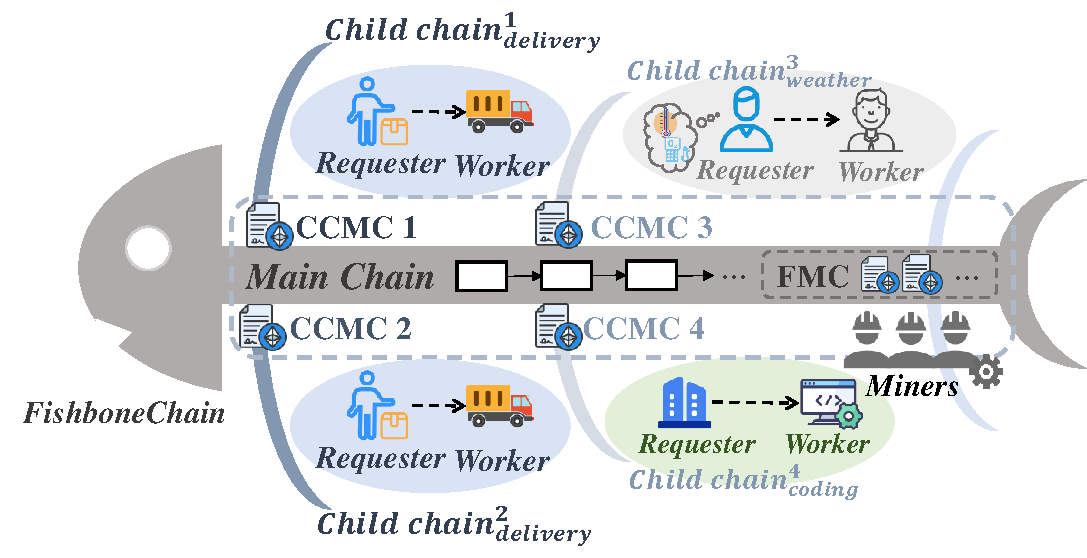
\includegraphics[width=1.0\linewidth]{system_model.pdf}
    \caption{FishboneChain architecture}\label{fig:FishboneChain_architecture}
\end{figure}

Specifically, there are four child chains in Fig.~\ref{fig:FishboneChain_architecture}, with different colors representing different industries. Among them, Child chain 1 and 2 are both responsible for collecting delivery information, which can be expanded again if there is a performance bottleneck. Child chain 3 is responsible for collecting weather information. Child chain 4 is responsible for outsourcing coding work. They are managed by CCMC1-4 on the main chain respectively. In addition, there are many FMCs on the main chain created by requesters to publish tasks and settle the payment.

Next, we introduce our system model in detail.

\subsubsection{\textbf{Entities}}
There are four kinds of entities in our FishboneChain architecture: main chain miners, child chain miners, requesters, and workers. Generally speaking, miners maintain the blockchain, including the bidirectional synchronization between the main chain and child chains. Requesters post tasks with their specific requirements, and workers provide the needed services.
Below is a more detailed introduction on these entities:

\begin{itemize}
    \item \textbf{Miners.}
    All miners are responsible for maintaining the main chain. Besides, a group of miners can become child chain miners by establishing a child chain to process crowdsourcing tasks. They can earn more rewards by contributing to the efficient processing of crowdsourcing tasks in child chains. Those miners should periodically perform bidirectional synchronization between the main chain and the child chain.

    \item \textbf{Requesters.} Requesters post their tasks on the main chain and then leverage smart contracts to settle the rewards and manage their budget. They receive services from child chains.

    \item \textbf{Workers.} Workers receive task information from child chains and submit corresponding data or service receipts to these child chains. The data then undergoes a verification process to determine its validity. Upon successful verification, workers receive rewards on the main chain.
\end{itemize}

\subsubsection{\textbf{Blockchains}}

The FishboneChain architecture consists of one main chain and multiple child chains. Generally speaking, the main chain is used to post tasks, process fund transactions, and manage child chains. Child chains are used to process data submission, verification, and storage. A detailed description of the interaction between the main chain and child chains can be found in Section \ref{subsec:crowdsourcing_processes} and Section \ref{subsec:childchain_management}.

\begin{itemize}
    \item \textbf{Main chain:}
    The main chain is a publicly accessible, permissionless blockchain, similar to Ethereum, that supports financial transactions and smart contracts. It manages users' assets, maintains a ledger of the statuses of all child chains, issues tasks, and processes transactions.

    \item \textbf{Child chain:}
    A child chain is a compact blockchain established and maintained by a group of miners from the main chain to process data submission, verification, and storage for crowdsourcing tasks. Multiple distinct child chains can be established to accommodate the diverse requirements of various crowdsourcing tasks. Each child chain can be tailored to specific needs through the customization of data structures, cryptographic algorithms, consensus mechanisms, and other relevant parameters.

\end{itemize}


\subsubsection{\textbf{Smart Contracts}}\label{subsub:smartcontract}
There are three types of smart contracts, which used to manage child chains, funds and tasks.
\begin{itemize}
    \item \textbf{Child Chain Management Contract (CCMC)}:
    A CCMC represents a child chain. CCMC manages the deposit of its own child chain miners, periodically records data digests of the child chain, and deals with the malicious miners on the child chain.

    \item \textbf{Fund Management Contract (FMC)}: An FMC, which manages a list of task management contract (TMC) and two balances, free balance $FB$ and locked balance $LB$, is created by a requester to post tasks and manage fund settlement. FMC is responsible for automating the management of requester's funds and the activation of tasks through two balances $FB$ and $LB$. The details are presented in Section \ref{pay_bills}.
    \item \textbf{Task Management Contract (TMC)}: A TMC not only contains the specific task requirements, budgets per epoch and other parameters, but also is implemented with specific verification algorithm to identify predefined malicious behaviors. The definition and role of the verification algorithm are presented in Section \ref{subsubsec:dispute_resolution}.
\end{itemize}


\subsection{Security Assumptions}\label{subsec:security_assumption}
    The overall security of the FishboneChain architecture primarily depends on the security of the main chain. We assume that honest miners control more than $51\%$ of the total stake on the main chain which implements a Proof of Stake consensus mechanism like Ethereum. This assumption is crucial for maintaining the integrity of the fund settlement and task management processes that occur on the main chain. We assume that there will be malicious requesters attempting to perform double-spending attacks on the child chains by posting crowdsourcing tasks on multiple child chains when they lack sufficient funds. Regarding child chains, we assume that an adversary can gain control over a child chain for up to $m$ epochs by compromising the majority of the miners in that child chain. After $m$ epochs, the honest miners of the compromised child chain will regain control of their own child chain nodes, causing the adversaries to lose control over the child chain. At this point, rational workers, requesters and child chain miners can detect the malicious behavior and exit the child chain.

\subsection{Design Goals}\label{subsec:design_goals}

Our primary objective is to propose a scalable and flexible blockchain-based crowdsourcing platform that supports various task allocation, worker recruitment, incentive mechanisms, and privacy-preserving protocols. In particular, the FishboneChain crowdsourcing platform has the following security and performance design goals.

\subsubsection{\textbf{Security Goals}}
As a crowdsourcing platform, the security of funds and data are both crucial, which include:
\begin{itemize}
    \item \textbf{Child Chain Immutability}
            During the collecting slot of an epoch in the child chain, the child chain is responsible for gathering the execution results of crowdsourcing tasks. Verified results are stored in child chain blocks. In the subsequent syncing slot, the digest of generated blocks is uploaded to the corresponding CCMC on the main chain. Even if the child chain is compromised, the contents of blocks whose digest are stored in CCMC can not be tampered with.
    \item \textbf{Fund security.}
          The security of funds encompasses two aspects: first, safeguarding requesters' funds against theft resulting from blockchain attacks, and second, resisting double-spending attacks by malicious requesters that will prevent workers and child chain miners from receiving their rightful payments.
\end{itemize}

\subsubsection{\textbf{Performance Goals}}

The widespread adoption of blockchain applications is hindered by the constraints of scalability and compatibility, while fund liquidity poses another challenge when applying child chains to crowdsourcing scenarios. 
Therefore, the system's performance must meet the following goals:

\begin{itemize}
    \item \textbf{Scalability.}
          The proposed architecture should support a massive number of users and large-scale data in the crowdsourcing scenarios. In addition, it should be capable of enhancing system throughput as the system load increases.
    \item \textbf{Compatibility.}
          The proposed architecture should be able to accommodate a variety of crowdsourcing scenarios. Specifically, it should support a variety of task allocation and privacy-preserving mechanisms as well as adjust consensus mechanisms, block structures, \textit{etc.}
    \item \textbf{Fund liquidity.}
          Users can flexibly manage their funds and freely transfer funds between different tasks as needed. The smart contract automatically manages the budgets for tasks, and the balance of the budget is recycled after the task is settled. As long as there are sufficient funds, users can post tasks on all child chains without having to manage multiple locked and non-interoperable funds.
\end{itemize}


\section{Proposed solution}\label{section:solution}

\subsection{Overview} \label{subsec:overview}

We propose FishboneChain, a blockchain-based crowdsourcing platform that achieves scalability, compatibility, and guaranteed liquidity. Our platform features a structure comprising a main chain and multiple child chains. We divide our scheme into two parts: the crowdsourcing process and the child chain management. The crowdsourcing process primarily describes how requesters post tasks, child chain miners collect tasks, workers submit task results on the child chain, and finally, child chain miners submit task results to receive rewards. Then, it is followed by the child chain management process, which includes child chain establishment and participation, dispute resolution and child chain termination.

In the rest of this section, we detail the crowdsourcing process and the child chain management process of the proposed architecture. After that, we explain the mechanisms for enhancing the throughput of the architecture.

\subsection{Crowdsourcing Processes on FishboneChain}\label{subsec:crowdsourcing_processes}

As shown in Fig.~\ref{fig:crowdsourcing_detail}, the crowdsourcing process consists of four steps: Post tasks, Collect tasks, Submit and verify data and Pay bills.

\begin{figure}[htbp]
    \centering
    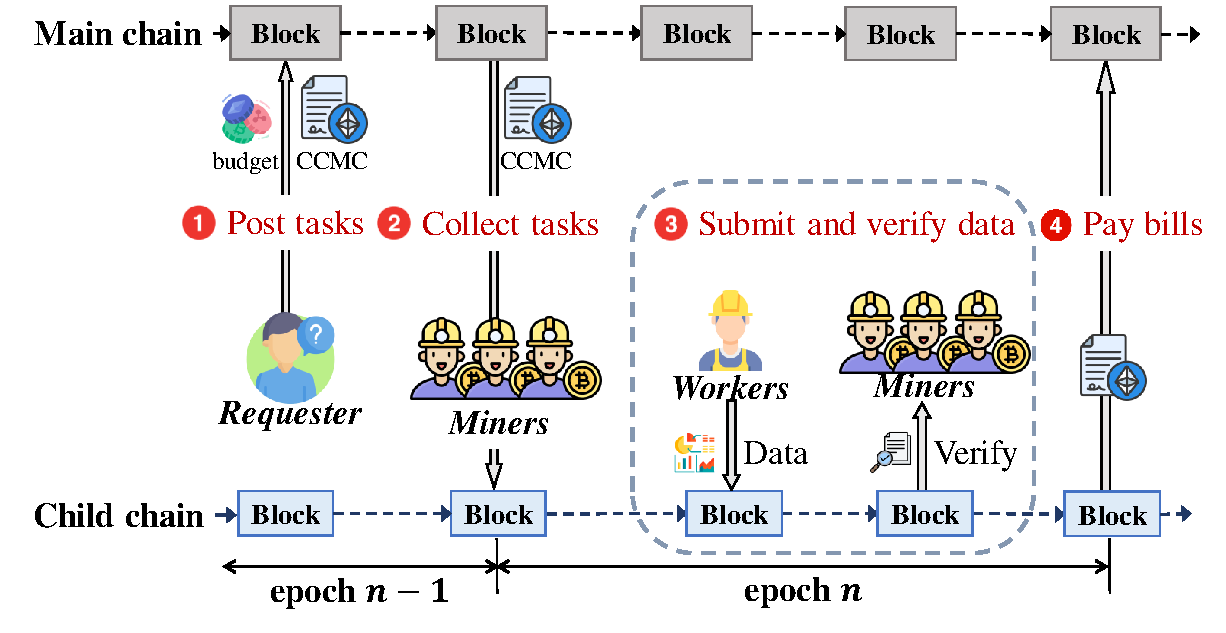
\includegraphics[width=1.0\linewidth]{crowdsourcing_detail.pdf}
    \caption{Crowdsourcing Details on FishboneChain}\label{fig:crowdsourcing_detail}
\end{figure}

\subsubsection{\textbf{Post Tasks}}\label{post_tasks}

Requesters start the task posting process on the specific CCMC on the main chain. To initiate a new task, a requester is required to establish at least one FMC on the main chain, transferring a fund to serve as the task's budget. Notably, a single FMC can oversee the budgets of multiple tasks. Then, the requester can proceed to post the task on the FMC. The task itself must contain specific requirements, including data packaging and verification mechanisms, alongside the budget allocated for a single epoch on the child chain, denoted as $B$. The requester should also declare the CCMC's address to designate the responsible child chain for task processing. Upon initial posting, the task assumes a default state of $\mathsf{terminated}$. Requesters can invoke FMC to activate tasks. FMC determines this by checking the relationship between $FB$ and $B$. If $FB > B$, it indicates that the free balance of FMC is sufficient to cover the budget for this task in the next epoch. In this case, the task status is adjusted $\mathsf{activated}$. Otherwise, the state of this task remains $\mathsf{terminated}$. Since the decision to activate a task is made by FMC automatically through a comparison of $FB$ and $B$, instead of being set by the requesters themselves, this can prevent double-spending attacks by malicious requesters.


\subsubsection{\textbf{Collect Tasks}}\label{collect_tasks}

The next step involves child chain miners gathering tasks from the main chain and recording them onto the respective child chain. At this moment, the child chain operates within the syncing slot and no longer generates new blocks. Child chain miners collect all tasks assigned to their child chain with the status of $\mathsf{activated}$ from all FMCs on the main chain. Then, miners collaborate to establish consensus on the list of new tasks. Once the consensus is reached, this list is packed into blocks at the beginning of the next epoch.

\subsubsection{\textbf{Submit, Verify and Store Data}}

The third step involves both workers' data submission and miners' verification and storage processes. Workers select appropriate crowdsourcing tasks based on their capabilities and task requirements, guided by information recorded on the child chain. Then workers submit data in accordance with the specifications outlined by the corresponding child chain. After confirming that the task's budget is sufficient and the data meets the requirements, miners work toward consensus for each task. Once consensus is reached, the task data provided by workers is recorded into the newly generated block on the child chain. Although this paper does not focus on the privacy-preserving issues of crowdsourcing, it's worth noting that our platform aligns well with various blockchain-based privacy-preserving schemes for crowdsourcing, such as \cite{wang2022triple,cai2019towards,koutsos2021agora}. Workers can encrypt their crowdsourcing data using cryptographic parameters specified by the requester. The data is collected and verified by child chain miners only when the task's budget for an epoch is adequate. As an illustration, consider a scenario where a requester posts a traffic crowdsourcing task on a child chain soliciting 100 pieces of traffic information. In this example, even if the 101st piece of data is valid, miners would refrain from collecting it if the budget for the task's epoch has been exhausted.

\subsubsection{\textbf{Pay Bills}}\label{pay_bills}

In the final step, the requesters settle bills with the workers. First, child chain miners initiate the process by generating bills for tasks managed during the current collecting slot. Then, these miners submit the data index and task bills for the completed crowdsourcing tasks to the respective FMC on the main chain. Once the FMC confirms that the bill remains within the preset budget limit, it proceeds with updating the task's status and distributing rewards to both workers and child chain miners. The FMC first deducts the billed amount from $LB$ and transfers any remaining funds to $FB$. After that, the FMC determines the task's state based on the amount of $FB$. If $FB$ is sufficient to meet the task's budget $B$ required for the next epoch, the FMC transfers $B$ from $FB$ to $LB$ and designates the task's status as $\mathsf{activated}$. Otherwise, the task's state is set to $\mathsf{terminated}$. The requester can transfer funds to FMC to reactivate this task. After that, the FMC proceeds to allocate rewards to the accounts of workers and child chain miners on the main chain, utilizing funds from $LB$. Finally, FMC returns the state of the task for the next epoch.

\begin{figure}[htbp]
    \flushleft
    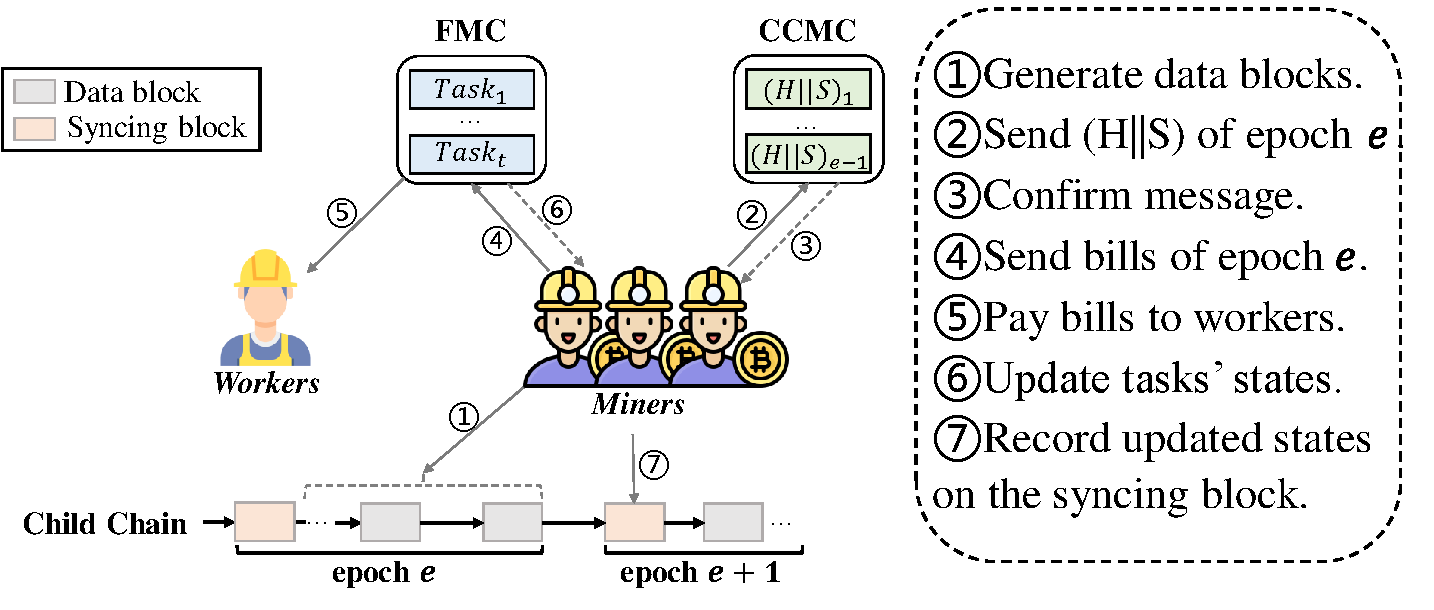
\includegraphics[width=1\linewidth]{pay_bills.pdf}
    \caption{The process of paying bills.}\label{fig:pay_bills}
\end{figure}

Child chain miners collect the information of all activated tasks that are posted on their child chain and record them in the child chain's syncing block, marking the beginning of the next working epoch. The FMC determines the task's state based on the available amount of $FB$ and assigns rewards from $LB$, thereby safeguarding against potential double-spending attacks. On the other hand, the FMC reallocates any surplus budget to the $FB$, effectively maintaining fund liquidity. The system's architecture permits requesters to efficiently manage multiple task budgets via the FMC, eliminating the necessity for them to immobilize numerous deposits on the main chain. This significantly alleviates the financial pressure on requesters during task posting. Moreover, the unutilized portion of a task's budget is routinely returned to the FMC's $FB$, allowing these funds to be used in other crowdsourcing tasks. This embodies the liquidity feature of our architecture.

For example, we assume that there are $k$ tasks during the collecting slot, represented as $T_1, T_2,\dots, T_k$. Every task $T_j$ is linked to a fund management contract $FMC_j$, where $j = 1,2,\dots ,k$. Initially, miners compute a data digest of recently generated blocks during $S_c$, represented as $H$. Subsequently, they compute a bill for every task, represented as $B_1, B_2,\cdots, B_k$. Every bill contains the rewards of miners and workers and their corresponding payment addresses. Next, all miners generate aggregate signatures on the bills, represented as $AS_h$,$AS_{B_1}, AS_{B_2},\cdots, AS_{B_k}$. Finally, $M^c$ submits $H$ and $AS_H$ to CCMC, and submits $B_i$ and $AS_{B_i}$ on the corresponding FMC.

After receiving $B_i || AS_{B_i}$ on the main chain, the FMC verifies the aggregated signature and then checks whether the total amount of the bill exceeds the budget $B$. If the signature is valid and the bill is within the budget, TC invokes the FMC to assign rewards according to the bill. In the meantime, the TC sets its status as $\mathsf{waiting}$ and waits for the FMC to determine the status according to the FMC's balance.

There are two kinds of fund balance in an FMC: free fund balance $FB$ and locked fund balance $LB$. Every time the requester transfers a fund to FMC, it is directly added to the free fund balance $FB$. Then, the requester can invoke the FMC to activate or reactivate a task. In the following, we present the interaction between child chain miners and FMC in the syncing slot as an example to describe the details of fund management. The child chain miners submit a bill to FMC during the collecting slot. Since the task budget is already locked in $LB$, the FMC can pay the bill directly. After that, the FMC returns the remaining funds to $FB$. Finally, the status of the task in the next epoch is determined by the $FB$ and the budget. If the balance is bigger than the budget, the task will remain $\mathsf{activated}$, and FMC will transfer the budget $B$ from $FB$ to $LB$. Otherwise, the task will be $\mathsf{terminated}$.

\subsection{Child Chain Management}\label{subsec:childchain_management}
In this section, we present the details of child chain management, including how to establish a new child chain, how to join a child chain, how to resolve disputes, and how to terminate a child chain.

\subsubsection{\textbf{Child Chain Establishment}}

Main chain miners who share similar business requirements for crowdsourcing and aspire to attract more users and collect more data to enhance their business quality can assemble as a cohesive unit to establish a child chain. These child chain miners collectively deliberate and determine the parameters of the newly formed child chain based on their respective business contexts. This includes factors such as the choice of consensus mechanism and crowdsourcing protocols. For instance, miners involved in location services can configure a suite of task allocation strategies, worker recruitment tactics, incentive mechanisms, and privacy-preserving protocols tailored to their child chain. Due to the shared business backgrounds among child chain miners, the child chains can adopt efficient consensus mechanisms akin to those seen in consortium blockchains, including Delegated Proof of Stake (DPoS) and Practical Byzantine Fault Tolerance (PBFT). Furthermore, they must agree upon the duration of the collecting slot ($S_c$) in accordance with the real-time demands of their business. As shown in Fig.~\ref{fig:FishboneChain_architecture}, in scenarios like delivery, tasks are often processed on a daily basis, leading to a setting of $S_c$ at 24 hours. However, in weather information crowdsourcing scenarios, where timely data is of the essence, a shorter $S_c$ is often needed.

Following thorough negotiations, miners proceed to instantiate a fresh Child Chain Management Contract (CCMC) on the main chain and record their public details there. Each child chain miner commits a predetermined fund as a security deposit. If any miners engage in misconduct, other miners can eliminate them from the network and deduct their security deposit.

\subsubsection{\textbf{Child Chain Participation}}

Individuals on the main chain interested in contributing to a child chain can initiate the registration process. To make informed decisions, users can access the Child Chain Management Contracts (CCMCs) stored on the main chain, which provide comprehensive information about the child chain. This empowers users to select and engage with a child chain aligned with their preferences. Given that requesters and workers aren't actively engaged in the child chain's consensus mechanism, their registration process remains straightforward. Requesters and workers simply generate a key pair and submit their public key to the designated child chain. On the other hand, honest miners are crucial for ensuring the child chain's security. As a result, miners intending to participate in a child chain must secure unanimous agreement from all existing miners within that child chain. Following consensus attainment, the new miner proceeds to deposit funds into the CCMC, which grants the new miner permission to participate in the child chain and access to historical block data shared by other miners on the same child chain.

\subsubsection{\textbf{Dispute Resolution}}\label{subsubsec:dispute_resolution}
We categorize disputes into two types: standard verifiable disputes and non-standard disputes. Standard verifiable disputes are disputes that can be predefined and the corresponding verification algorithms are encoded into the smart contract at the time of CCMC or TMC deployment. The child chain miners or requesters can submit a verification request to the CCMC or TMC. These verification algorithms are usually computationally expensive. Child chain miners or requesters should pay a fee to cover the cost. Child chain miners or requesters should submit the data to be verified and the signatures of child chain miners from the child chain consensus process. The corresponding CCMC or TMC automatically performs the verification algorithm. If violations are found, the relevant miners' deposits are transferred to the requester. This process is fully transparent and verifiable, with severe penalties serving as an effective deterrent against malicious behavior.

Non-standard disputes are difficult to verify through predefined algorithms, such as when child chain miners interfere with or attack the consensus process. A CCMC voting mechanism is employed. When signatures from miners exceed a preset threshold, the suspected malicious miner can be expelled from the child chain. To prevent abuse of this mechanism by malicious users, the expelled miner's deposit is returned. This mechanism balances punishment and protection, contributing to the healthy development of the child chain ecosystem. This mechanism leverages the advantages of smart contract automation while retaining the flexibility of human judgment, effectively addressing various potential dispute scenarios.

\subsubsection{\textbf{ Child Chain Termination}}\label{subsubsec:terminate}

In cases where malicious miners form the majority, whether through attacks or corruption, honest miners, requesters, or workers can terminate the child chain by submitting a complaint to the CCMC. Besides, if child chain miners unanimously agree to terminate the child chain due to strategic requirements, they must collect an aggregate signature from all miners concerning the termination request and then submit the request and signature to the CCMC. The CCMC verifies the aggregated signature. If it is valid, the CCMC enacts the termination process, discontinuing the reception of data digests from all miners and refunding the security deposit to each miner.


\section{Security analysis }\label{section:security_analysis}
In this section, we present a security analysis of the FishboneChain system. We demonstrate that it meets the security design goals outlined in section \ref{section:system_model}, namely fund security and data integrity. As a precursor, we first conduct a theoretical analysis of FishboneChain in terms of child chain security, followed by a sequence of proof for fund security and data integrity.

\subsection{Child chain Security}

Firstly, we give a theoretical analysis of FishboneChain in terms of child chain security, which encompasses both immutability and firewall property. 

\begin{theorem}\label{thm_child_chain_immutability}

    \textbf{Child Chain Immutability.} Let $\mathcal{H}: \{0,1\}^* \rightarrow \{0,1\}^n$ be a second pre-image resistant hash function, and let $\mathcal{MT}: \{B_1, \dots , B_m\} \rightarrow \{0,1\}^n$ denote a Merkle Tree construction algorithm that processes blocks $B^j_1, B^j_2, \dots, B^j_{n_j}$ generated during epoch $\mathsf{j}$ and outputs a Merkle Tree root $R^j \in \{0,1\}^n$ as the epoch digest. For each block $B^j_i$, let $MP^j_i$ represent its corresponding Merkle proof. The CCMC on the main chain implements a Merkle proof verification function $\mathcal{MPV}$, which takes $(B^j_i, MP^j_i, R^j)$ as input and returns a bool value. Specifically, $\mathcal{MPV}(B^j_i, MP^j_i, R^j) = \text{true}$ if and only if the hash of $B^j_i$ combined with $MP^j_i$ successfully verifies against the Merkle Tree root $R^j$.

    Consider an adversary $\mathcal{A}$ that gains control of a child chain $\mathcal{C}$ at epoch $\mathsf{e}$. For any block $B^j_i$ in previous epochs $\mathsf{j} \in [0, e-1]$ and $i \in \{1, \dots, n_j\}$, the adversary $\mathcal{A}$ is incapable of executing either of the following attacks:
    \begin{itemize}
    \item Forging a block $B'^j_i$ and providing a corresponding Merkle proof $MP'^j_i$ and with the root $R^j$ on CCMC such that $\mathcal{MPV}(B'^j_i, MP'^j_i, R'^j) = \text{true}$.
    \item Altering the stored root $R^j$ to $R'^j$ within the CCMC in a manner that allows a forged block $B'^j_i$ to pass the $\mathcal{MPV}$ verification, i.e., $\mathcal{MPV}(B'^j_i, MP'^j_i, R'^j) = \text{true}$.
    \end{itemize}
\end{theorem}

\begin{proof}
    Assume that the adversary $\mathcal{A}$ can forge a block $B'^j_i$ along with a corresponding Merkle proof $MP'^j_i$ such that $\mathcal{MPV}(B'^j_i, MP'^j_i, R^j) = \text{true}$. This implies that $\mathcal{H}(B'^j_i)$, combined with $MP'^j_i$, produces a valid path to the Merkle root $R^j$. However, since $\mathcal{H}$ is a second pre-image resistant hash function, it should be computationally infeasible for $\mathcal{A}$ to find a different block $B'^j_i \neq B^j_i$ that hashes to the same value required to validate against $R^j$. Therefore, successfully forging such a block and proof would violate the second pre-image resistance property of $\mathcal{H}$.

    Suppose the adversary $\mathcal{A}$ can alter the stored Merkle root from $R^j$ to $R'^j$ within the CCMC such that a forged block $B'^j_i$ passes verification, i.e., $\mathcal{MPV}(B'^j_i, MP'^j_i, R'^j) = \text{true}$. Achieving this requires $\mathcal{A}$ to change the state of the main chain's CCMC. Given that the main chain operates under a Proof-of-Stake (PoS) consensus mechanism where more than half of the stake is held by honest participants, the security of the main chain ensures that an adversary cannot unilaterally alter contract states without controlling a majority of the stake. Therefore, successfully altering $R^j$ would imply that $\mathcal{A}$ has breached the PoS assumptions, specifically that they control more than half of the total stake, which contradicts our security assumptions.
\end{proof}

\begin{theorem}\label{thm_child_chain_firewall}
\textbf{Firewall Property.}

In the FishboneChain architecture, consider a set of child chains $\{\mathcal{C}_1, \mathcal{C}_2, \dots, \mathcal{C}_s\}$, each operating its own consensus protocol $\Pi_k$ with miners $\mathcal{M}_k$ and maintaining ledger $\mathcal{L}_k$. Suppose an adversary $\mathcal{A}$ can compromise at most one child chain at any given time. If $\mathcal{A}$ compromises child chain $\mathcal{C}_i$ at time $t$, then for any other child chain $\mathcal{C}_j$ with $j \ne i$, the sequence of transactions $\sigma_j$ that appears in $\mathcal{C}_j$ is a valid execution according to its consensus protocol $\Pi_j$. Specifically, $\sigma_j$ is a valid projection of some word from the asset validity language onto the ledger $\mathcal{L}_j$, ensuring the integrity and correctness of $\mathcal{L}_j$ despite the compromise of $\mathcal{C}_i$.
\end{theorem}

\begin{proof}
Each child chain $\mathcal{C}_k$ operates independently with its own consensus protocol $\Pi_k$, miner set $\mathcal{M}_k$, and ledger $\mathcal{L}_k$. There is no direct communication or shared state between different child chains; interactions occur only through the main chain's Child Chain Management Contract (CCMC), which enforces strict isolation.

Given that the adversary $\mathcal{A}$ has compromised $\mathcal{C}_i$ by controlling enough miners in $\mathcal{M}_i$ to subvert its consensus protocol $\Pi_i$, their influence is confined to $\mathcal{C}_i$. Since $\mathcal{A}$ is limited to compromising at most one child chain at a time, they lack control over the miner set $\mathcal{M}_j$ of any other child chain $\mathcal{C}_j$. Without sufficient influence in $\mathcal{M}_j$, the adversary cannot manipulate the consensus protocol $\Pi_j$ or affect the validation and ordering of transactions in $\mathcal{C}_j$.

The consensus protocol $\Pi_j$ ensures that only valid transactions, as defined by the asset validity language, are appended to the ledger $\mathcal{L}_j$. Therefore, the sequence of transactions $\sigma_j$ processed by $\mathcal{C}_j$ is a valid execution that adheres to the protocol rules and maintains ledger consistency. The miners in $\mathcal{M}_j$, following $\Pi_j$, collectively agree on the ledger updates, and the integrity of $\mathcal{L}_j$ is preserved.
\end{proof}

\subsection{Fund Security}
We then prove that FishboneChain satisfies fund security by demonstrating its resilience against double-spending attacks and showing that the potential financial loss for each participant is limited.

\begin{theorem}\label{thm_anti_double_spending}
    \textbf{Double-Spending Resistance.} Let $\mathcal{A}$ be a malicious requester who intends to publish $k$ tasks $\{T_1, T_2, \dots, T_k\}$ on child chains.  Each task $T_i$ requires a budget of $B_i$ in an epoch. If the free balance ($FB$) of $\mathcal{A}$ in the FMC less than $\sum_{i=1}^k B_i$, $\mathcal{A}$ cannot successfully activate all $k$ tasks. 
\end{theorem}

\begin{proof}

    Assume that the adversary $\mathcal{A}$ attempts to activate the tasks sequentially from $T_1$ to $T_k$. For each task $T_i$, the activation process involves invoking the FMC, which checks whether $\mathcal{A}$ has sufficient funds to cover the budget $B_i$. The FMC deducts $B_i$ from the free balance ($FB$) upon successful activation of $T_i$. Since $FB < \sum_{i=1}^k B_i$, there must exist an index $t \in \{1, \dots, k\}$ such that: $FB \geq \sum_{i=1}^{t-1} B_i \quad \text{and} \quad FB < \sum_{i=1}^t B_i.$ This means that $\mathcal{A}$ has enough funds to activate the first $t-1$ tasks but lacks sufficient funds to activate task $T_t$.

    If $\mathcal{A}$ attempts to activate $T_t$ despite the insufficient $FB$, the FMC's logic should prevent this activation by performing a balance check and rejecting the transaction due to inadequate funds. The only way for $\mathcal{A}$ to bypass this restriction is to either:
    \begin{itemize}
        \item Tamper with the FMC's Logic: Modify the smart contract code of the FMC to disable or alter the balance checking mechanism, allowing activation without sufficient funds.
        \item Alter $FB$: Illegitimately increase $FB$ within the FMC to reflect a higher balance than what $\mathcal{A}$ actually possesses, thus passing the balance check.
    \end{itemize}

Any attempt by $\mathcal{A}$ to tamper with the FMC or alter $FB$ without proper authorization would violate the main chain's security assumptions and immutability guarantees. Therefore, unless $\mathcal{A}$ can compromise the main chain by controlling a majority of the stake—which contradicts our security assumptions—the adversary cannot successfully activate task $T_t$.

\end{proof}

\noindent\textbf{Limited financial loss:}
    Let $\mathcal{C}$ be a child chain compromised by an adversary $\mathcal{A}$ during the period $[t, t + m ]$ epoch. 
    The financial loss for each participant is limited. 
 
\noindent\textbf{1) Workers:} For any worker $w$ who completes $N_w$ tasks during the compromised period, with a maximum reward per task of $R_{\max}$, the maximum financial loss $L_w$ satisfies:
    \begin{equation}
        L_w \leq R_{\max} \cdot N_w.
    \end{equation}
    During the compromised period, the adversary $\mathcal{A}$ may manipulate task results or reward distributions, potentially causing honest workers to lose their expected compensation. The worst-case scenario for a worker $w$ is that they receive no rewards for tasks completed during the compromised period. Let $N_w$ be the number of tasks completed by worker $w$, and $R_{\max}$ be the maximum reward per task. The maximum financial loss $L_w$ for worker $w$ is therefore: $ L_w \leq R_{\max} \cdot N_w$. Rational workers can detect anomalies such as lack of rewards or irregularities in task validation results. Upon detection, they will cease participation in the compromised child chain to prevent further losses, effectively limiting their maximum loss to the tasks already completed during the compromised period.

\noindent\textbf{2) Requesters:} For any requester $r$ who allocates a budget of $B_{epoch}$ per epoch for their tasks, the maximum financial loss $L_r$ satisfies:
    \begin{equation}
        L_r \leq B_{epoch} \cdot m.
    \end{equation}
    An adversary controlling $\mathcal{C}$ can interfere with task execution by providing low-quality or fabricated results while consuming the requester's budget. However, rational requesters monitor the quality of task results and can detect significant degradation. Let $B_{epoch}$ be the budget allocated by requester $r$ per epoch. Given the synchronization mechanism between the main chain and child chains occurs at epoch boundaries, a requester can respond to detected issues by terminating or suspending tasks on the compromised chain at the end of the current epoch. The maximum financial loss $L_r$ for requester $r$ over $m$ compromised epochs is thus: $L_r \leq B_{epoch} \cdot m $. 
    
\noindent\textbf{3) Honest miners:} For any honest miner $v$, with expected mining rewards of $M_{epoch}$ per epoch, the maximum financial loss $L_v$ satisfies:
    \begin{equation}
        L_v \leq M_{epoch}.
    \end{equation}
    Honest miners may suffer losses if they are excluded from block production due to the adversary manipulating the consensus protocol of $\mathcal{C}$. They may not receive expected mining rewards during the compromised period. Let $M_{epoch}$ be the expected mining rewards per epoch for a miner. Rational miners monitor the consensus process and can detect abnormalities such as consistent failure to include their blocks or votes. Upon detecting such issues, an honest miner $v$ can choose to exit the compromised child chain. Since the security deposits of honest miners are managed by the main chain's Child Chain Management Contract (CCMC), these deposits are secure and retrievable upon exit. The maximum financial loss $L_v$ for miner $v$ is limited to the mining rewards of one epoch, accounting for the time needed to detect the compromise and take action: $L_v \leq M_{epoch}$. By withdrawing promptly, honest miners prevent further losses beyond the immediate compromised period.
    
\section{Performance Analysis}\label{section:performance_analysis}
In this section, we conduct a comprehensive performance analysis of our FishboneChain platform, focusing on two key aspects: overall system throughput with multiple child chains and the effectiveness of our fund management scheme.

\begin{table}[htbp]
    \centering
    \caption{Child chain's data throughput}
    \label{tab:childchain_throughput}
    \begin{tabular}{ccccccc}
        \toprule
        \noalign{\smallskip}
        number of nodes & 4     & 6     & 8     & 10    & 12    & 14    \\
        \midrule
        \noalign{\smallskip}
        throughput      & 478.7 & 443.9 & 415.6 & 401.1 & 384.2 & 375.2 \\
        \bottomrule
    \end{tabular}
\end{table}
We first evaluate the data throughput of a single child chain under different network sizes to establish a baseline for our subsequent experiments.
In order to measure the data throughput on a child chain, we establish a child chain with multiple miners based on the FISCO BCOS with PBFT consensus. We conduct a benchmark test using Hyperleger Caliper. There are two E5-2690v3 CPUs (2.6GHz) and 100GB RAM on the server running on Debian Linux. As shown in Table~\ref{tab:childchain_throughput}, the throughput of the child chain decreases as the number of nodes increases. With 4 nodes, the system achieves the highest throughput of 478.7 transactions per second(tps), while with 14 nodes, the throughput drops to 375.2 tps. This decline is expected due to the increased communication overhead in the PBFT consensus as more nodes participate in the network. Based on these results, we set the child chain tps to 400 for our subsequent experiments, which represents a reasonable performance level for a child chain with approximately 8-10 nodes.

\subsection{Throughput Analysis}

\begin{table}[htbp]
    \centering
    \caption{Notions for System}
    \begin{tabular}{cl}
        \toprule
        \makecell[c]Notions & Meaning                                          \\
        \midrule
        $tps_m$             & tps of the main chain                            \\
        $tps_c$             & tps of a child chain                             \\
        $k$                 & number of tasks in one epoch $E$                 \\
        $b$                 & amount of data collected for a task              \\
        $h$                 & transactions on the child chain in one epoch $E$ \\
        \bottomrule
        \label{tab:notions_throughput}
    \end{tabular}
\end{table}


We now analyze how our FishboneChain architecture improves overall system throughput. Table~\ref{tab:notions_throughput} summarizes the key notations used throughout this section. Let $tps_m$ represent the throughput of the main chain, and $tps_c$ represent the throughput of a child chain. In our analysis model, we consider a working epoch $E$ containing $k$ tasks, denoted as $T_1, T_2, \dots, T_k$.

\begin{figure}[htbp]
    \centering
    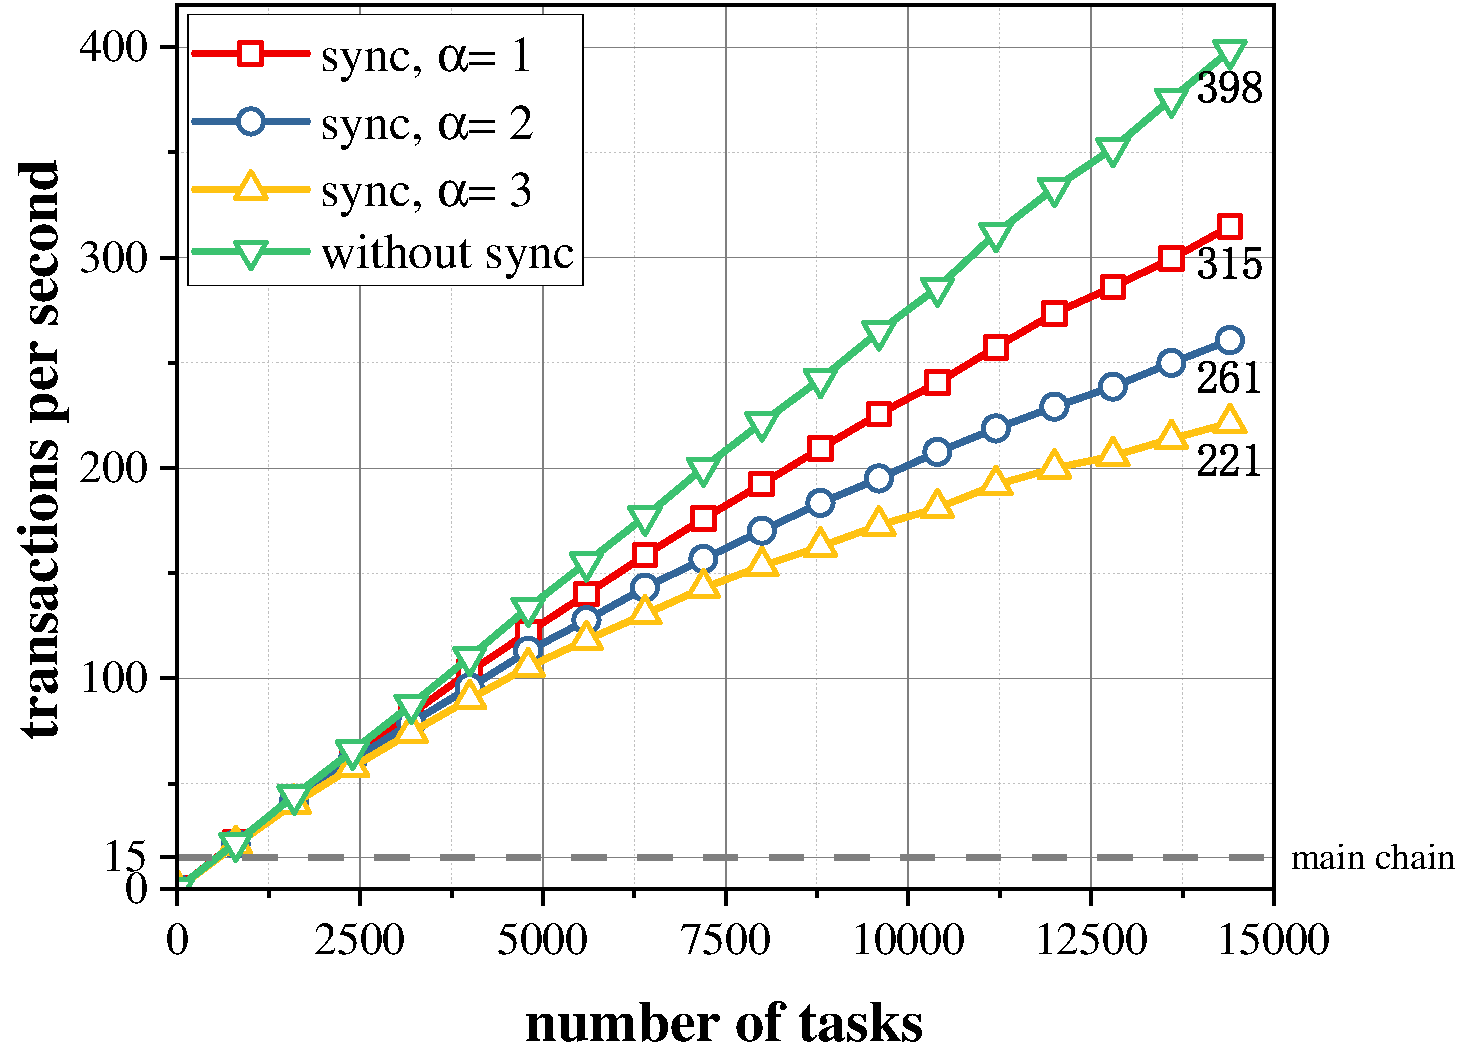
\includegraphics[width=0.88\linewidth]{epoch-tps.pdf}
    \caption{Throughput comparison between the main chain, child chain without sync, and different $\alpha$ for child chains in one epoch}
    \label{fig:epoch-tps}
\end{figure}

We demonstrate the impact of the syncing slot $S_s$ on the throughput of a child chain within one epoch. A child chain's epoch consists of two slots: the collecting slot, denoted as $S_c$, and the syncing slot, denoted as $S_s$. We assume that $S_c$ consists of $k$ tasks denoted as $T_1, T_2, \dots, T_k$, where each task $T_i$ involves $b_i$ transactions per epoch. Without loss of generality, we assume that $b_i$ follows a normal distribution with parameters $(b_m,b_{sd})$. In the collecting slot, the total number of transactions, denoted as $h$, is equal to $\sum_{i=1}^k b_i$ transactions. We have $h = \sum_{i=1}^k b_i$, $h_{max} = tps_c \cdot S_c$ and $k_{max} = \frac{h_{max}}{b_m}$. During the syncing slot, the child chain miners submit bills and digest of the child chain to the main chain. Therefore, the duration of the syncing slot is related to the number of tasks and the throughput of the main chain. So we define that $S_s = \frac{\alpha k}{m}$. Since the throughput of Ethereum is limited to $12-15$ tps, if multiple child chains submit transactions simultaneously, the length of the syncing slot is extended. We use $\alpha$ to represent the number of child chains present in the sync slot, with values ranging from 1 to 3 in our analysis to model different levels of synchronization congestion. Therefore, with an epoch, the tps of a child chain is $\frac{h}{S_c+ S_s} = \frac{\sum_{i=1}^k b_i}{S_c + \frac{\alpha k}{m}}$. Based on the above implementation and analysis, we set $tps_m = 15, tps_c =400, b_m = 100, S_c = 3600 $. Therefore, $h_{max} = 1440000, k_{max} = 144000$. As shown in Fig.~\ref{fig:epoch-tps}, with this parameter setting, the child chain's tps remains significantly higher than the main chain's tps. Then we can conclude that the syncing slot does not have much effect on the tps of the child chain.


\begin{figure}[htbp]
	\centering
	\subfigure[Child chain throughput as tasks posting rate increase with different $b_m$]{
            \label{fig:child_chain_multi_epoch_1}
			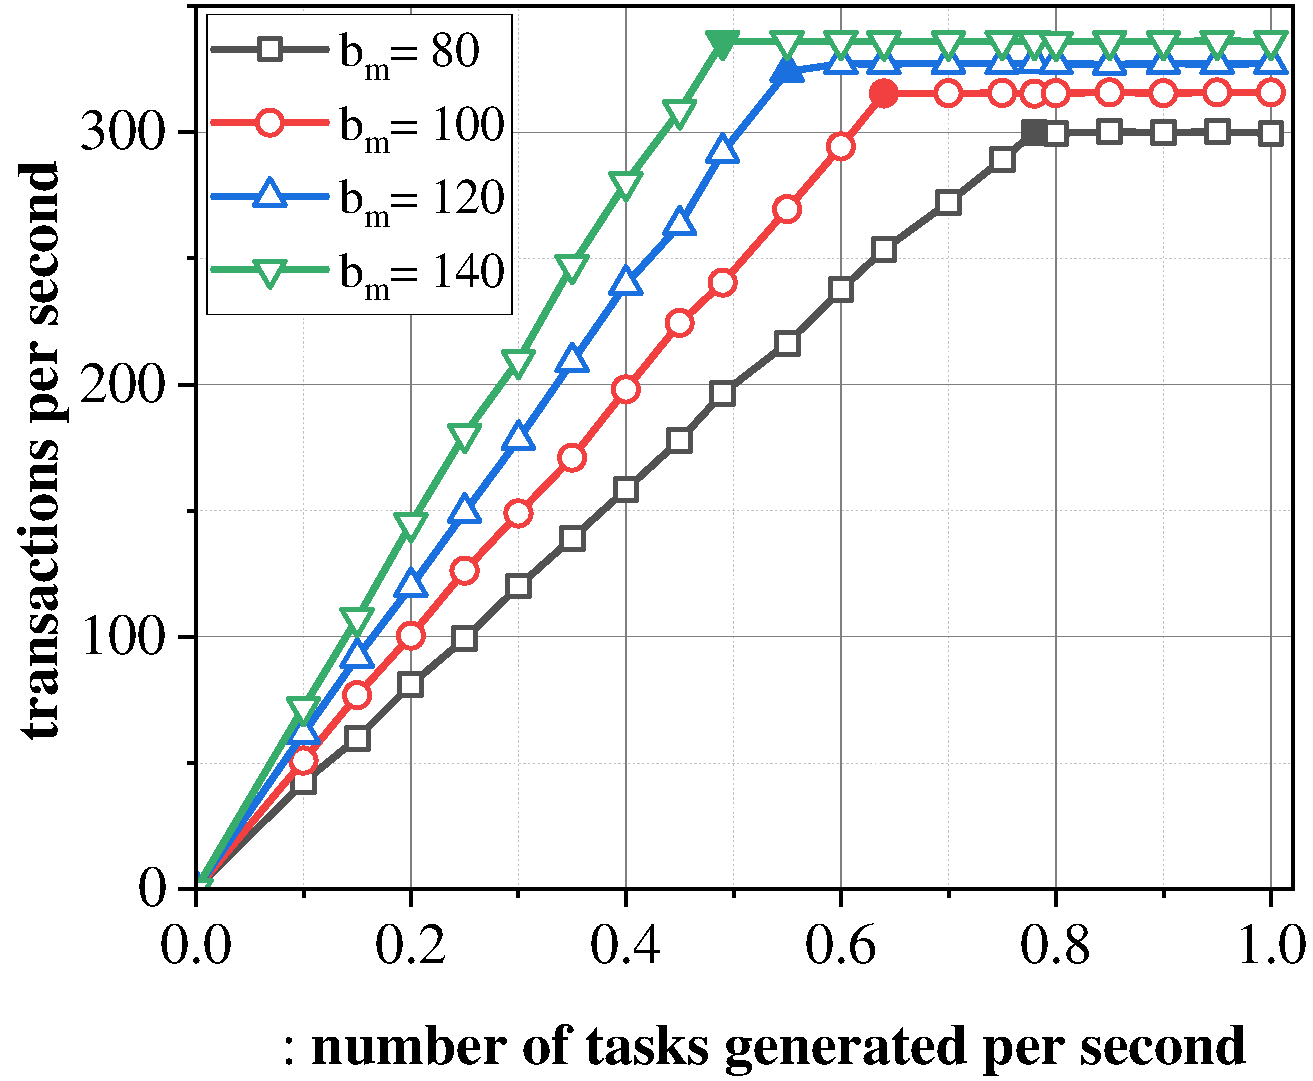
\includegraphics[width=0.466\linewidth]{data-lamda-tps-figure.pdf}
	}
    \subfigure[Child chain throughput as tasks posting rate increase with different $e_m$]{
            \label{fig:child_chain_multi_epoch_2}
            \centering
   		 	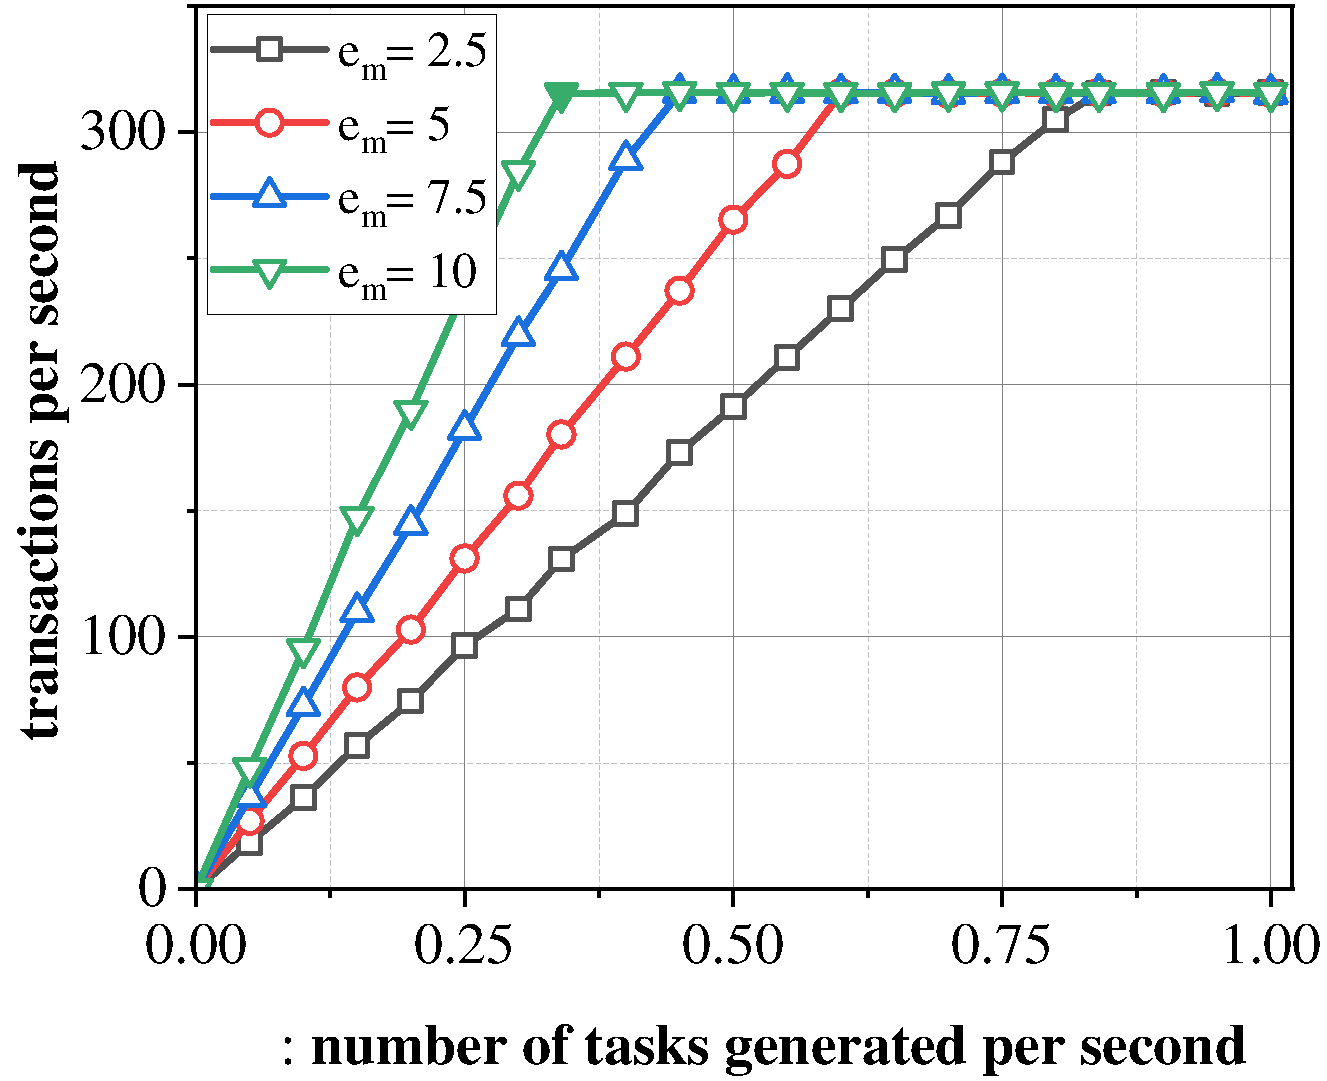
\includegraphics[width=0.466\linewidth]{slot-lamda-tps-figure.pdf}
    }\\

	\subfigure[Child chain load as tasks posting rate increase with different $b_m$]{
            \label{fig:child_chain_multi_epoch_3}
            \centering
			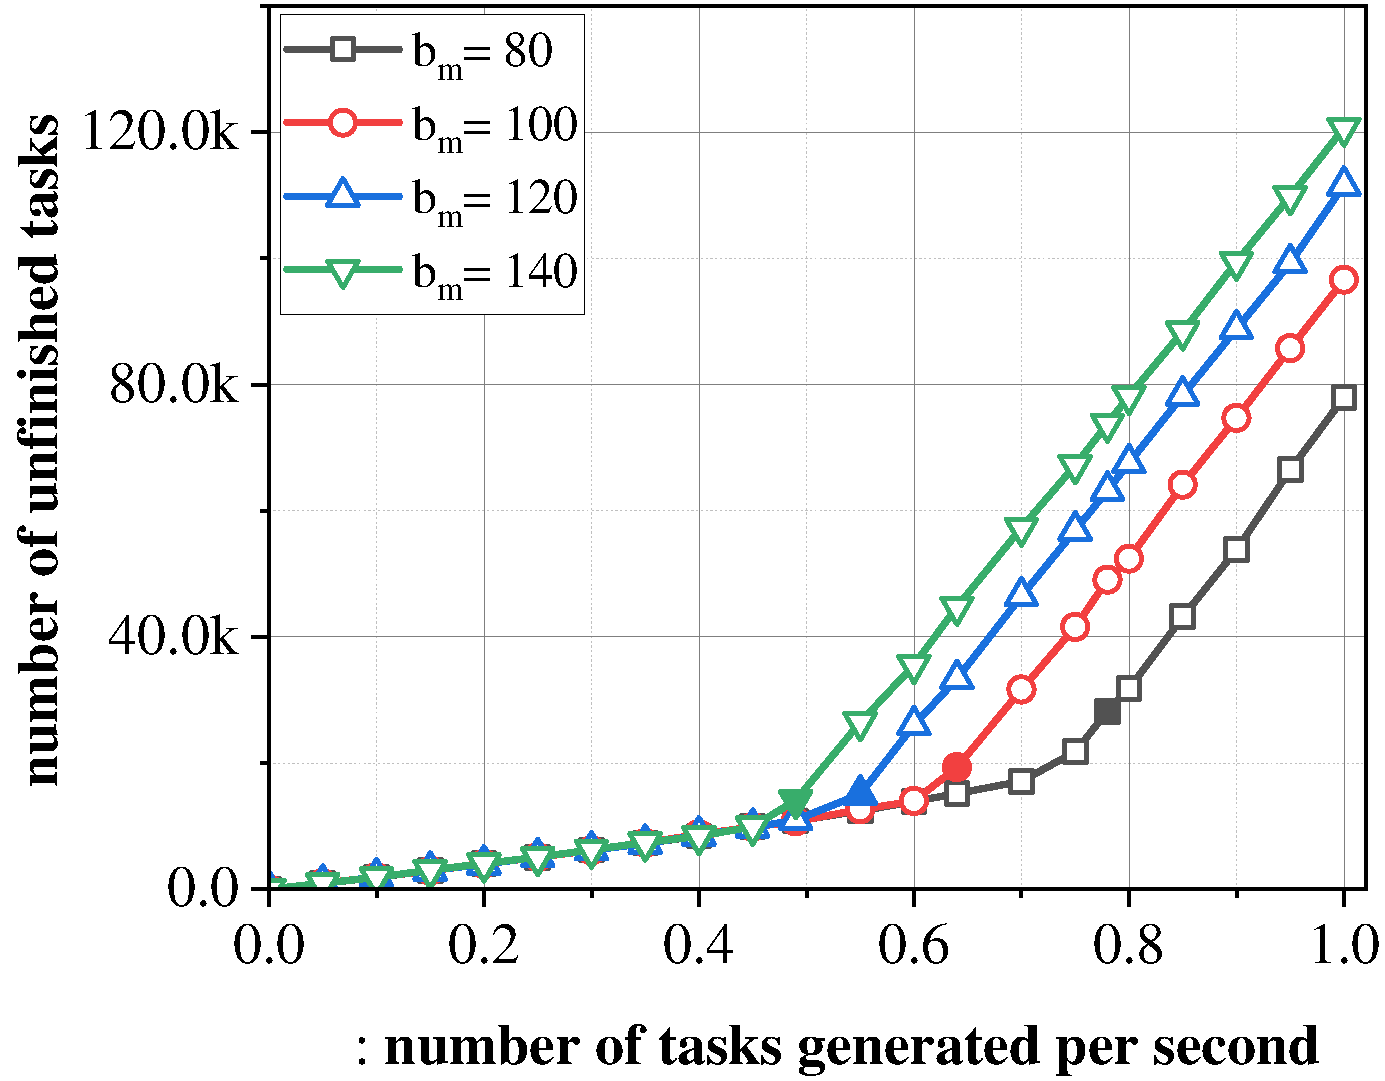
\includegraphics[width=0.466\linewidth]{data-lamda-tasks-figure.pdf}
	}
    \subfigure[Child chain load as tasks posting rate increase with different $e_m$]{
            \label{fig:child_chain_multi_epoch_4}
            \centering
		 	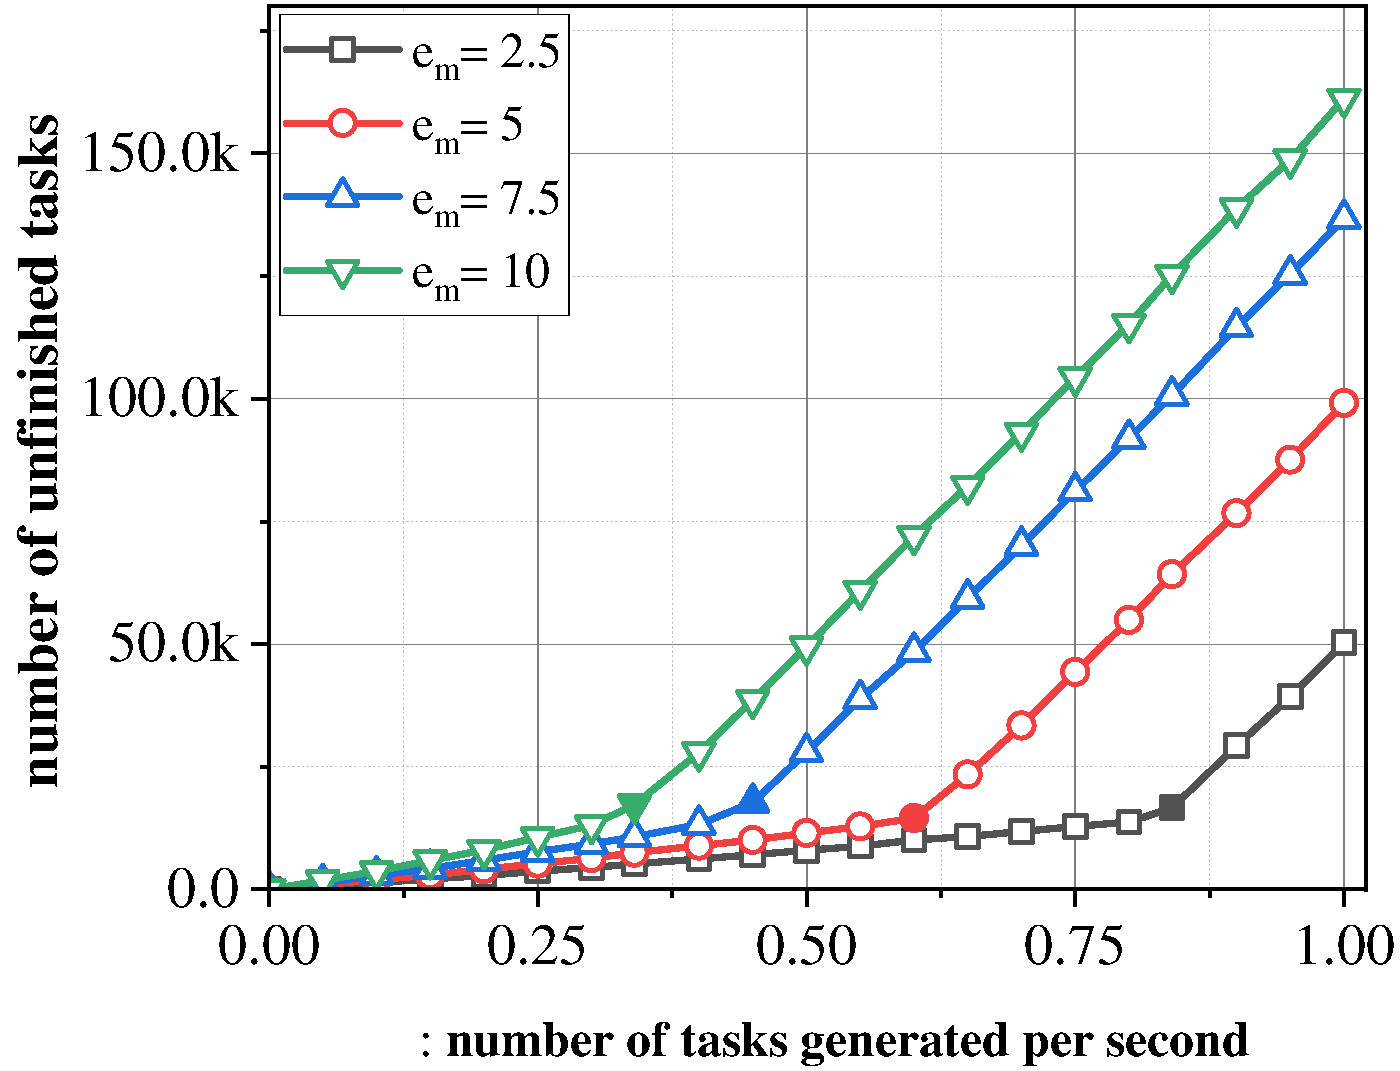
\includegraphics[width=0.466\linewidth]{slot-lamda-tasks-figure.pdf}
    }
	\caption{Child chain throughput and load as tasks posting rate increase in multiple epochs}
	\label{fig:child_chain_multi_epoch}
\end{figure}
To further investigate the performance characteristics of child chains, we assess their stable throughput across multiple epochs under varying task loads.
The evaluation encompasses two fundamental aspects: transactions per second (tps) and the number of unfinished tasks. The tps represents the child chain's maximum load capacity, and the number of unfinished tasks indicates its current load status. We model the task generation process using a Poisson distribution, where $\lambda$ represents the task posting rate. Additionally, the epochs for task $T_i$ are represented as $e_i$, which follows a normal distribution of $(e_m, e_{sd})$. The duration of the syncing slot is determined by $k$, while the current epoch's task count $k$ depends on the task generation rate $\lambda$ and the duration of the preceding epoch. When $\lambda$ remains constant, the child chain's throughput reaches a steady state across multiple epochs. Consequently, for a specific $\lambda$, we collect the child chain's tps and the count of unfinished tasks after 50 epochs. This set of graphs illustrates the throughput and workload of child chains under varying task generation rates, examining the effects of transaction count per task ($b_m$) and execution cycles ($e_m$).


We first examine the impact of different parameters on the maximum throughput of a child chain. As shown in Fig.~\ref{fig:child_chain_multi_epoch_1}, as the task generation rate $\lambda$ increases, the throughput of the child chain grows linearly before plateauing. Higher $b_m$ values lead to earlier saturation and higher maximum throughput, indicating that the higher the number of transactions required per task within one epoch $b_m$, the higher throughput the child chain can achieve. However, this simultaneously corresponds to a lower number of tasks it can support. As shown in Fig.~\ref{fig:child_chain_multi_epoch_2}, the average number of epochs required for each task does not affect the maximum throughput of the child chain, but only influences the task capacity of the child chain. Specifically, the fewer epochs a task requires, the more tasks the child chain can handle simultaneously. Then we investigate how different parameters affect the number of tasks that the child chain can successfully handle. Fig.~\ref{fig:child_chain_multi_epoch_3} demonstrates that the growth rate of tasks successfully processed by child chains is not affected by the number of transactions required per task within one epoch. However, the higher the number of required transactions, the fewer tasks can be processed. Fig.~\ref{fig:child_chain_multi_epoch_4} demonstrates that as the number of epochs required for a task increases, the number of tasks that can be successfully processed by the child chain decreases. Additionally, the child chain reaches its limit more quickly.

\begin{figure}[htbp]
    \centering
    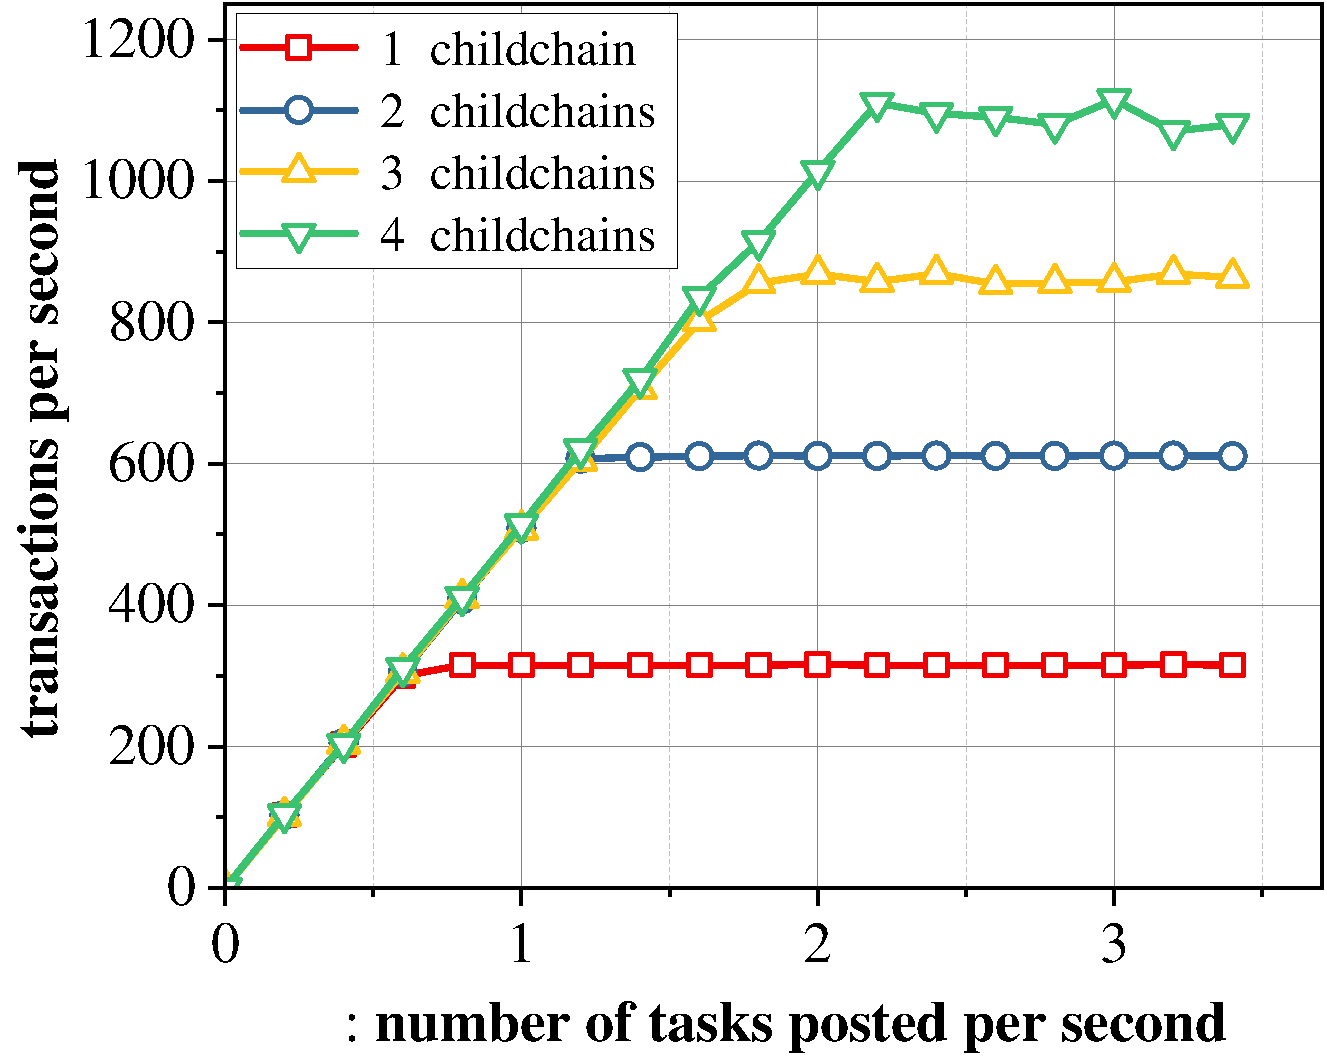
\includegraphics[width=0.88\linewidth]{multi-cc-lamda-tps-4-figure.pdf}
    \caption{System throughput with multiple child chains}
    \label{fig:multi-chain}
\end{figure}

After examining the performance of individual child chains, we proceed to evaluate the throughput of the entire FishboneChain platform with multiple child chains as the task generation rate increases. We set the tps of the main chain to 15 and the epoch length of each child chain to 3000 seconds, 3600 seconds, 4000 seconds and 4800 seconds to simulate the different parameters of child chains. As shown in Fig.~\ref{fig:multi-chain}, the tps of our platform expands as the number of child chains increases and eventually reaches its maximum value at four child chains, at which point it maxes out at around 1100.

After reaching around 1100 transactions per second, the tps of the main chain becomes the primary bottleneck, limiting the overall throughput of our platform. In the meantime, with the continuous development and maturation of technologies such as sharding, the tps of the main chain is expected to improve. To thoroughly investigate the maximum throughput potential of the platform system, we set the main chain tps within the range of 10-100 and conduct experiments to determine the maximum number of supported child chains and the corresponding total throughput under various main chain tps conditions. As shown in Fig.~\ref{fig:max_tps}, as the main chain tps continues to increase, the number of child chains and the maximum tps of the platform also increases linearly. When the main chain tps reaches 100, the platform can support 25 child chains and the maximum tps of the platform is reaching around 10000. These results demonstrate that our platform possesses significant performance scalability potential. Even a modest increase in the main chain's tps can facilitate the addition of multiple child chains, resulting in a substantial boost to the platform's overall throughput, potentially by several thousand. This underscores the platform's efficient architecture and its capacity for considerable expansion with relatively minor enhancements to the main chain's performance. Fig.~\ref{fig:max_tps} serves as a crucial reference framework for the architectural design and scalability planning of real-world crowdsourcing platforms. This performance mapping provides platform architects with precise guidance on system configuration requirements. For instance, when a platform's anticipated transaction volume approaches 10,000 transactions per second, our results demonstrate that maintaining a main chain processing capacity of at least 100 tps is essential to ensure operational stability and service quality. This insight is particularly valuable for large-scale crowdsourcing platforms with user bases in the millions, where transaction demands can fluctuate dramatically. The architectural flexibility illustrated in our results enables significant economic advantages through resource optimization. Platform designers can implement a cost-effective scaling strategy by maintaining moderate main chain performance while dynamically adjusting the number of child chains to accommodate changing demands. Furthermore, our architecture provides a progressive scaling pathway suitable for platforms at various growth stages. Emerging crowdsourcing applications can begin with minimal configurations, like lower main chain tps and fewer child chains, and scale incrementally as their user base expands. 


\begin{figure}[htbp]
    \centering
    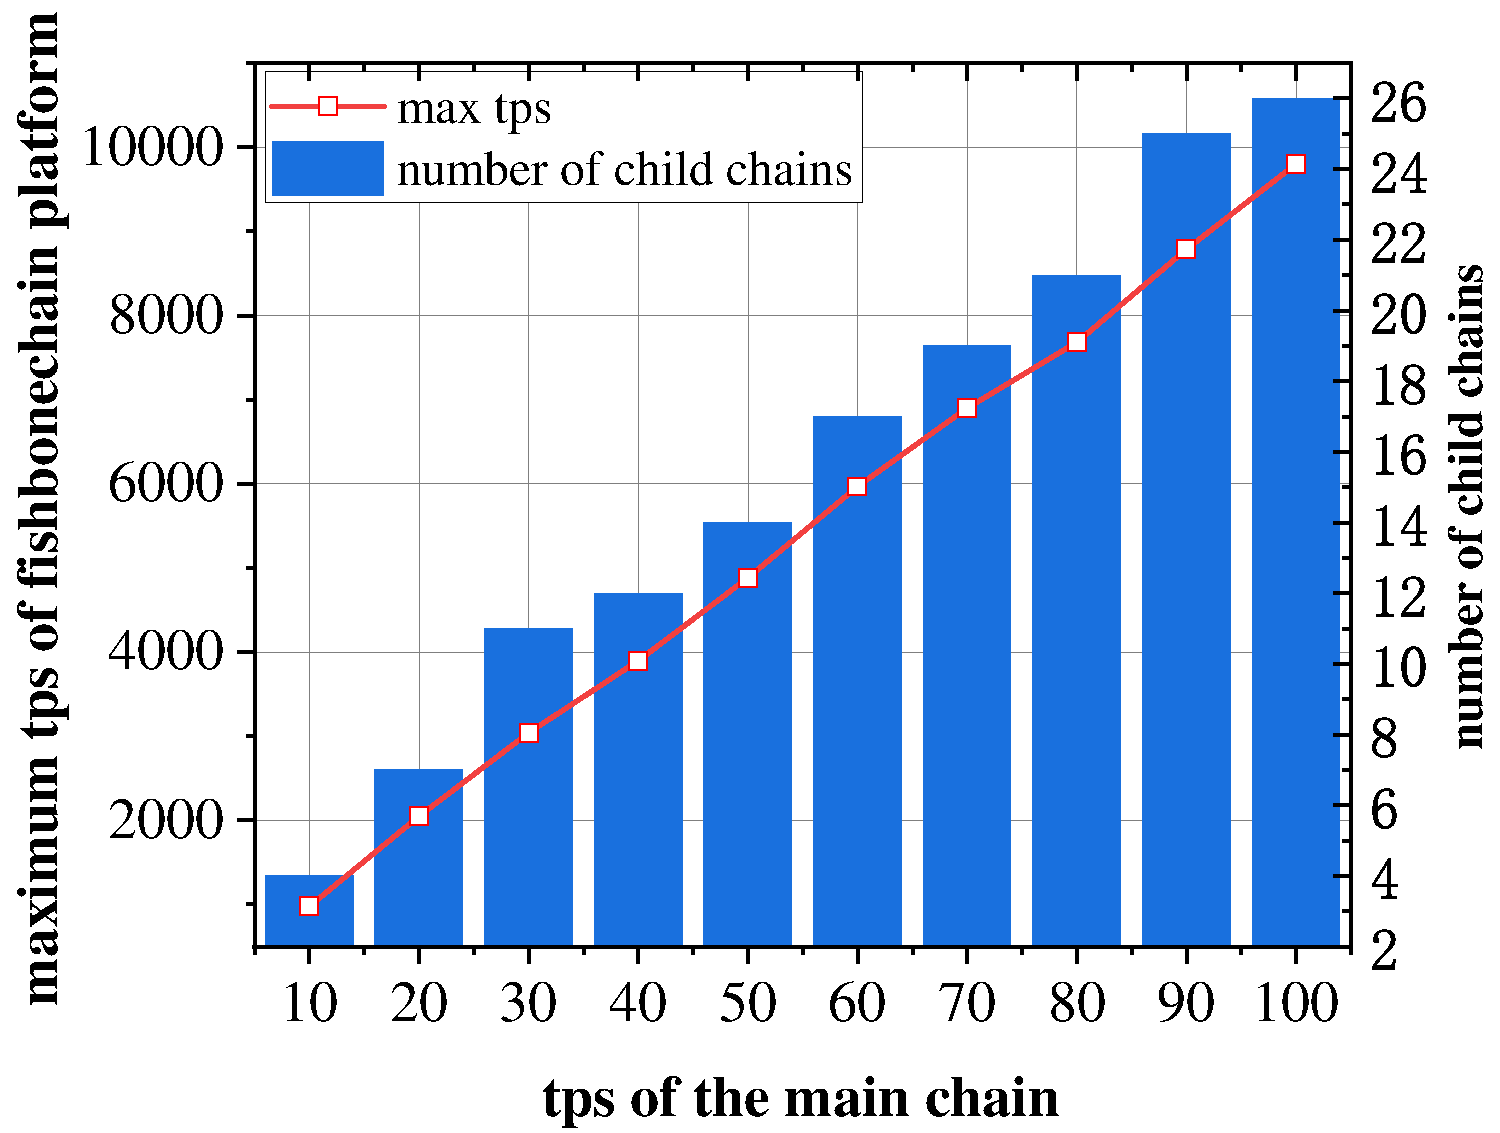
\includegraphics[width=0.88\linewidth]{max-tps.pdf}
    \caption{Platform performance when tps of the main chain increase}\label{fig:max_tps}
\end{figure}

\subsection{Analyse of Fund Management Scheme}
we now turn our attention to the analysis of our novel fund management scheme, designed to address the challenges of fund fragmentation and liquidity in multi-chain crowdsourcing platforms. In state-of-the-art blockchain platforms with multiple child chains or sidechains, to prevent double-spend attacks, users have to lock a fund on the main chain for every child chain or sidechain. However, when users lock multiple funds on the main chain to access multiple child chains at the same time, it will lead to fund fragmentation and reduce the liquidity of funds. We address these challenges with a new fund management mechanism tailored for crowdsourcing scenarios. First, we mitigate the issue of fund fragmentation by implementing two fund balances in FMC: the free fund balance $FB$ and the locked fund balance $LB$. At the beginning of a child chain epoch, a budget $B$ is transferred from $FB$ to $LB$ to prevent requesters from performing double-spending attacks. When rewards are assigned to miners and workers at the end of a child chain period, any remaining fund fragment resulting from the difference between the budget ($B$) and the total bill amount ($\mathsf{Bill.amount}$) is added into the free fund balance $FB$. Therefore, after each reward assignment, the fund fragment is transferred to $FB$ for future tasks.

To quantitatively compare the locked fund percentages between our periodic fund management scheme and the traditional approach during task execution, we design a simplified scenario for analysis. In the baseline scheme, requesters are required to lock individual budgets at the beginning of the task, leading to a potentially substantial accumulation of frozen funds. By contrast, our FishboneChain architecture permits requesters to periodically transfer funds to FMC for budget management in any time, mitigating the locked fund issue. To compare locked fund percentages between the two schemes during task execution, we design a simplified scenario for analysis. Assuming there are $s$ child chains with the same duration of epoch and a requester posts a task on each of them. Each task demands $t$ epochs for completion, and the budget per task is $b$. For the baseline, the requester should lock $L=tb$ for every task separately, which is a $s*t*b$ for frozen funds. For the baseline scheme, the requester needs to lock $L = tb$ funds for each task separately, resulting in a total initial locked amount of $L_{total} = s * L = s * t * b$. In the $i$-th period of $t$ periods, where $i \in [0,t)$, the frozen fund for each task is $F^{baseline}_i = (t-i)b$. In other words, at period $i=1$, the budget of each $T_i$ that is actively used is only $b$, while the remaining $F^{baseline}_1 = (t-1)b$, although not yet used, remains locked. At period $i=2$, the frozen fund for each task is $F^{baseline}_2 = (t-2)b$. At the last period ($i=t$), the frozen fund becomes $F^{baseline}_t = (t-t)b=0$, meaning all budgets are used in this period. Therefore, in the $i$-th period, the proportion of frozen funds in the total budget is $\frac{s*F^{baseline}_i}{s*L} = \frac{(t-i)b}{tb} = \frac{t-i}{t}$. Because the base scheme locks funds on the main chain, each is $tb$. For the convenience of analysis, in our scheme, the requester also locks the same fund $L=tb$ to the main chain at one time but periodically locks these funds in $s$ times. Therefore, at the $i$ epoch, $i \in [0,t)$, the total amount of locked funds is $F^{FishboneChain}_i =  t*b \cdot \lfloor 1+\frac{i}{t/s} \rfloor -i \cdot sb$
and the total amount of used funds is $i * sb$. Therefore, the locked fund percentage in the $i$ epoch is $\frac{F^{FishboneChain}_i}{t * s * b}= \{\lfloor1+\frac{i}{t/s}\rfloor \cdot \frac{t}{s}-i\}/t$.

\begin{figure}[htbp]
    \centering
    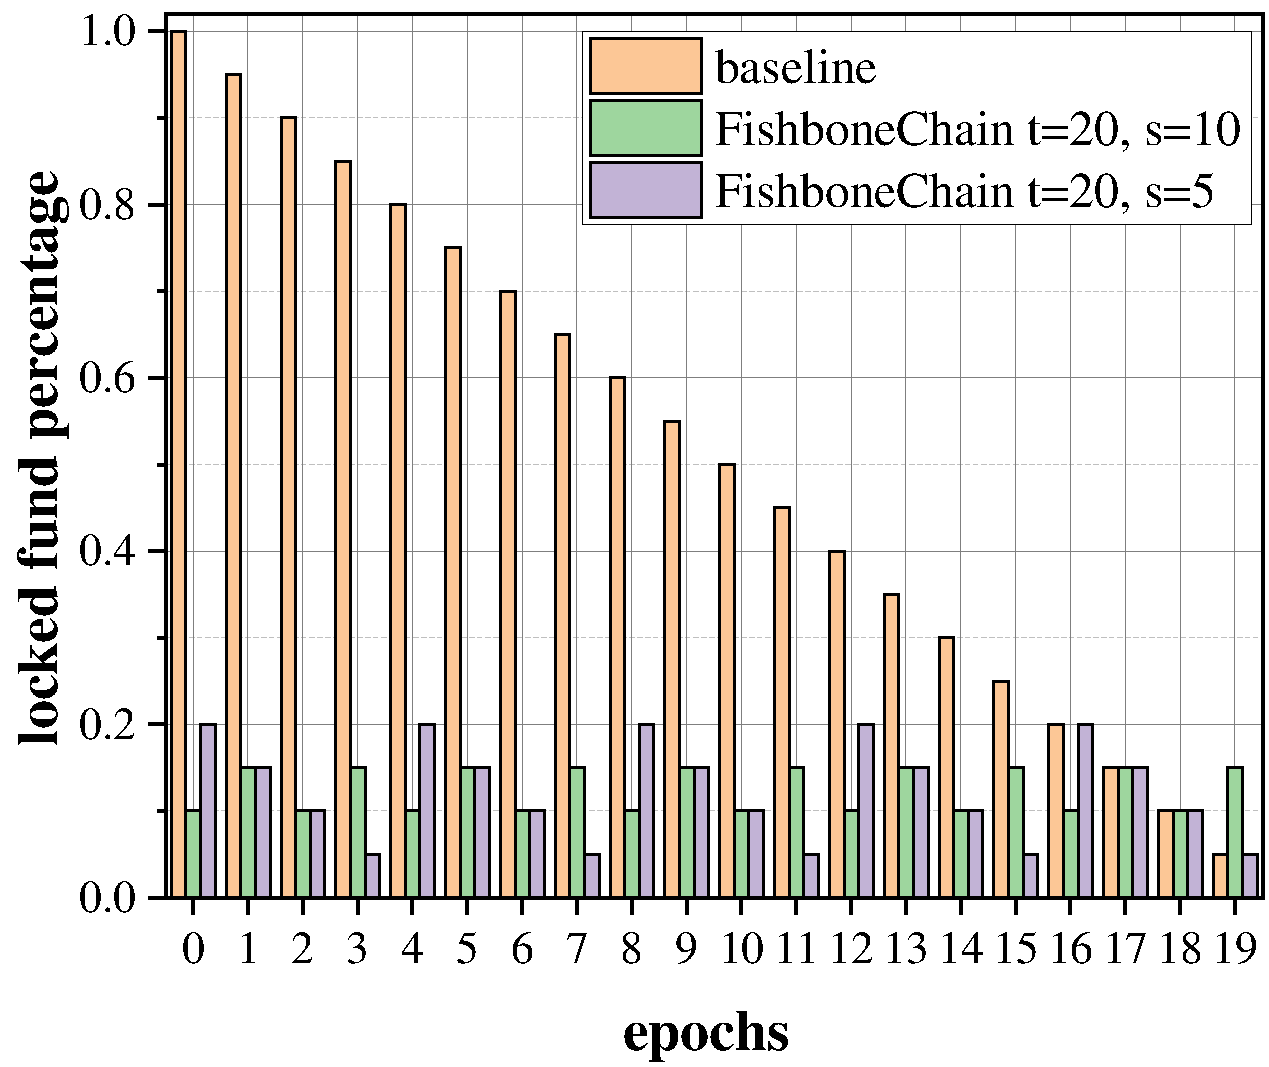
\includegraphics[width=0.88\linewidth]{locked_fund_comparison.pdf}
    \caption{Comparison of the percentage of locked funds}
    \label{fig:locked_fund_per}
\end{figure}

As shown in Fig.~\ref{fig:locked_fund_per}, the percentage of locked funds is shown for the baseline and our scheme, where two sets of parameters are set for our simplified FishboneChain scenario. The orange bar represents the baseline scheme, where the requester locks all budgeted funds on the blockchain at the beginning of the task. The green bar illustrates the scenario where the requester publishes 10 tasks on child chains, with each task requiring 20 epochs to complete. The purple bar depicts the scenario of 5 tasks posted on child chains, with each task also requiring 20 epochs for completion. The horizontal axis represents the current period, while the vertical axis shows the percentage of locked funds. It is clear that the percentage of locked funds in our scheme is consistently lower than the baseline scheme, which means that the funds are quickly applied to the task budget for the next epoch. Even if we adjust the number of tasks posted by the requester from 10 to 5, the percentage of locked funds is still less than or equal to $20 \%$. For example, in a data annotation project with 10 child chains, 20 epochs per task, and a \$500 budget per epoch, traditional schemes require locking \$100,000 upfront, while our periodic fund management scheme releases funds gradually. At 25\% completion, our approach only reserves \$15,000-\$20,000 compared to \$75,000 in the traditional approach, freeing substantial capital for other operations. Even in this simplified scenario, implementing a periodic fund management scheme significantly reduces requesters' financial burden. In practical applications with varying task quantities and epoch requirements, requesters can develop fine-grained strategies tailored to their specific needs. This reduced liquidity pressure enables requesters to post more tasks with the same amount of funds, collecting information more comprehensively. The resulting increased platform activity attracts more miners and workers, fostering a positive ecosystem cycle for our FishboneChain platform.

\section{Conclusion}\label{section:conclusion}
In this paper, we proposed a new blockchain-based crowdsourcing platform named FishboneChain, which offers enhanced efficiency, flexibility, and compatibility in crowdsourcing scenarios. The incorporation of child chains improves the scalability and compatibility of the platform. By harnessing trust and reduced scale within child chains, more efficient consensus mechanisms can be chosen, thereby enhancing the throughput. Furthermore, these child chains can use different cryptographic algorithms to achieve different privacy-preserving priorities for various crowdsourcing scenarios. We also separate the data management and the fund management on different chains. This entails the settlement of funds on the main chain for better security and the storage and verification of data on the child chain for enhanced scalability. However, the introduction of child chains also raises fund fragmentation challenges. To resolve them, We design a new periodic fund management mechanism, which not only increases fund utilization but also mitigates fragmentation. Evaluation results show that the FishboneChain architecture can increase the data throughput by hundreds of times. Security analysis demonstrates the robustness of our platform, assuring fund security and data integrity.

\section*{Acknowledgment}
This work is supported in part by Anhui Province Key Technologies Research \& Development Program under Grant No. 2022a05020050, the National Natural Science Foundation of China under Grant No. 62372425, and Youth Innovation Promotion Association of the Chinese Academy of Sciences (CAS) under Grant No. Y202093.

\bibliographystyle{IEEEtran}
\bibliography{FishboneChain}

\begin{IEEEbiography}[{\includegraphics[width=1in,height=1.25in,clip,keepaspectratio]{Photo-WentuoSun.pdf}}]{Wentuo Sun} received his Bachelor's Degree from the School of Cyber Science and Technology, University of Science and Technology of China (USTC), in 2020. He is currently working toward the Ph.D. degree in the major of Information Security with the School of Cyber Science and Technology, USTC. His research interests include Blockchain, Network security and Applied Cryptography.
\end{IEEEbiography}

\begin{IEEEbiography}[{\includegraphics[width=1in,height=1.25in,clip,keepaspectratio]{Photo-KaipingXue.pdf}}]{Kaiping Xue (M'09-SM'15)} received the bachelor's degree from the Department of Information Security, University of Science and Technology of China (USTC), in 2003 and received the Ph.D degree from the Department of Electronic Engineering and Information Science (EEIS), USTC, in 2007. From May 2012 to May 2013, he was a postdoctoral researcher with the Department of Electrical and Computer Engineering, University of Florida. Currently, he is a Professor in the School of Cyber Science and Technology, USTC. He is also the director of Network and Information Center, USTC. His research interests include next-generation Internet architecture design, transmission optimization and network security. His work won best paper awards in IEEE MSN 2017 and IEEE HotICN 2019, the Best Paper Honorable Mention in ACM CCS 2022, the Best Paper Runner-Up Award in IEEE MASS 2018, and the best track paper in MSN 2020. He serves on the Editorial Board of several journals, including the IEEE Transactions on Information Forensics and Security (TIFS), the IEEE Transactions on Dependable and Secure Computing (TDSC), the IEEE Transactions on Wireless Communications (TWC), and the IEEE Transactions on Network and Service Management (TNSM). He has served as a Guest Editor for many reputed journals/magazines, and he has also served as a track/symposium chair for some reputed conferences. He is an IET Fellow and an IEEE Senior Member.
\end{IEEEbiography}

\begin{IEEEbiography}[{\includegraphics[width=1in,height=1.25in,clip,keepaspectratio]{Photo-MeiqiLi.pdf}}]{Meiqi Li} received her B.S. degree in Information Security from School of Cyber Science and Technology, University of Science and Technology of China (USTC), in 2021. She is currently working toward the Ph.D. degree in the major of Information Security with the School of Cyber Science and Technology, USTC. Her research interests include Blockchain, Network security and Applied Cryptography.
\end{IEEEbiography}

\begin{IEEEbiography}[{\includegraphics[width=1in,height=1.25in,clip,keepaspectratio]{Photo-XinyiLuo.pdf}}]{Xinyi Luo} received her B.S. degree in Information Security from School of the Gifted Young, University of Science and Technology of China (USTC), in 2020. She is currently working toward the Ph.D. degree in the major of Information Security with the School of Cyber Science and Technology, USTC. Her research interests include Blockchain, Network security and Applied Cryptography.
\end{IEEEbiography}

\end{document}